\documentclass[11pt,a4paper]{article}
\usepackage{paramanu}
\usepackage{longtable}
\graphicspath{{../../paper/figures/}{../../simulation/results/}}
\setrunningtitle{PARAMANU Reclaimer: All Explained Here}
\hypersetup{pdftitle={PARAMANU Reclaimer: All Explained Here}, pdfauthor={Milind K. Patil}}
\setcounter{tocdepth}{2}

% A plain box for "in plain words" summaries
\newtcolorbox{plain}{enhanced,breakable,colback=gray!6,colframe=gray!55,
  title={In plain words},fonttitle=\bfseries\small,coltitle=black,colbacktitle=gray!20}
\newtcolorbox{wherecode}{enhanced,breakable,colback=green!4,colframe=green!45!black,
  title={Where to find it},fonttitle=\bfseries\small,coltitle=white}

\begin{document}
\thispagestyle{plain}

\begin{ptitle}
PARAMANU RECLAIMER\\[4pt] ALL EXPLAINED HERE
\end{ptitle}

\begin{psubtitle}
A complete companion to the paper:\\
everything we did, why, how, and what came out
\end{psubtitle}

\begin{pauthor}
Milind K. Patil\\
Syncaissa Systems Inc.\\
\texttt{syncaissa@outlook.com}
\end{pauthor}

\begin{pdate}
Companion to the paper version of 29 September 2026 (53 pages)
\end{pdate}

\begin{keyinsight}
\textbf{What this document is.} The paper \emph{PARAMANU Reclaimer: Atomize-First Recovery -- A Sealed Plasma Reactor from Landfill to the Periodic Table} states results compactly, as a journal paper must. This companion explains \emph{all} of it in detail and in plain language: every idea, every proof, every calculation, every number, every check, every mistake we found and fixed, and where each piece lives in the repository. If the paper is later shortened, nothing is lost: it is all here. Read it front to back as a guided tour, or jump to any section from the contents.
\end{keyinsight}

\bigskip
\noindent\textbf{How to read it.} Each chapter follows the paper's order. Grey boxes, \emph{In plain words}, give the idea without equations. Green boxes, \emph{Where to find it}, name the code, data and results files. Every number comes from the repository's results (\texttt{Results.txt} lists them all, regenerated from the code) or from a cited source. The step-by-step instructions to reproduce everything are in \texttt{HOWTOREPLICATE.txt}; the proofs are worked through, with exercises, in \texttt{docs/STUDENT\_GUIDE.md}.

\newpage
\tableofcontents
\newpage

%=====================================================================
\section{The Idea in One Page}
%=====================================================================
Every recycling system in use today sorts first. Magnets pull out steel, eddy currents aluminium, optical sorters plastics, and each stream goes to its own process. What cannot be sorted, the fine, mixed, contaminated residue that makes up most of an old landfill, is buried again, burned or capped. That residue is where most of the trace metals and most of the toxic elements hide, and it is why 34 of about 60 metals are recycled at end of life at rates below 1\% \citep{graedel2011}.

PARAMANU asks: \emph{if recovery must eventually happen at the level of atoms anyway, why sort objects at all?} Take a batch of residue, seal it in an airtight reactor with no chimney, and heat it with plasma torches until everything is gas. At that point the difference between a pizza box and a battery is gone; there is only a hot gas of the elements. Then cool it in steps. Each group of elements condenses at its own temperature, so the elements come out one band at a time: tungsten and titanium first; then iron with palladium, platinum and part of the gold; then silicon, nickel and copper with the rest of the gold; then salts, silver and lead; then zinc and cadmium; and at the cold end water, while mercury is caught in a trap and the fuel gases are drawn into cylinders. Nothing escapes.

We call this \textbf{Atomize-First} recovery, and the system that does it the \textbf{PARAMANU Reclaimer} (Plasma-Assisted Recovery And Mining of Atoms, Neutralizing Urban-waste; \emph{param\={a}\d{n}u} is Sanskrit for the atom, the ``ultimate particle'' of classical Indian philosophy). For the thinkers who first imagined matter as \emph{param\={a}\d{n}u}, the atom was the smallest building block of the world; PARAMANU applies that idea to the waste we have buried: take it apart completely, keep what is valuable, lock away what is harmful, and vent nothing to the air. The metals in a landfill were mined once, from ore; PARAMANU harvests them again, from the waste we buried.

The paper does four things with this idea:
\begin{enumerate}
\item \textbf{Defines the architecture} (Chapter~\ref{ch:arch}): pre-treatment, a sealed plasma hot zone, and a condenser train.
\item \textbf{Proves what physics allows} (Chapter~\ref{ch:math}): eight mathematical results, from ``no atom is lost'' to ``a catalyst cannot change the outcome''.
\item \textbf{Tests every claim with an open simulation} built on NASA thermochemical data (Chapters~\ref{ch:code}--\ref{ch:results}), which confirms some claims, corrects others and adds one hard constraint the original vision missed: the hot phase may last only tens of milliseconds.
\item \textbf{Checks the simulation itself} by every independent means available (Chapter~\ref{ch:verification}), finds and fixes its defects, and states exactly what is proven, what is verified, and what only experiments can show (Chapter~\ref{ch:feasibility}).
\end{enumerate}

\begin{plain}
Turn trash into gas in a sealed box, then cool it slowly enough that each element condenses in its own place. Keep the valuable ones, lock away the toxic ones, and vent nothing to the air. The mathematics says this is allowed; the simulation says where each element goes and how much energy it takes; the checks say the simulation is right; and only a real experiment can say whether a real machine behaves like the simulation.
\end{plain}

%=====================================================================
\section{Words Used in This Document}\label{ch:glossary}
%=====================================================================
\begin{longtable}{@{}>{\raggedright\arraybackslash}p{3.6cm}>{\raggedright\arraybackslash}p{11.2cm}@{}}
\toprule
\textbf{Term} & \textbf{Meaning} \\
\midrule
\endhead
Atomize-First & Take the whole residue apart into atoms (a gas) before separating anything; the opposite of Sort-First. \\
Sort-First & Today's practice: separate objects and materials mechanically, then treat each stream. Modelled in the paper as a baseline. \\
Feed & The material that enters the reactor: here, one wet tonne of excavated landfill residue (default composition in \texttt{feed.py}). \\
Pre-treatment & Optional removal of easily separated material (steel, aluminium) before the plasma, 0--30\% of the mass. Always includes making hazards safe. \\
Plasma heap & The residue after it has been taken fully into the gas phase. (At 2,890\,K it is only 0.02\% ionized: really a hot vapor heated by plasma torches.) \\
Closed-mass principle & Every atom that enters leaves through a labelled outlet; nothing goes to the air. \\
Band & A temperature range in which a group of elements condenses, with its own collector. Final bands: A ($\ge$2,600\,K), B (2,000--2,600), C (1,600--2,000), D1 (1,300--1,600), D2 (1,000--1,300), E (400--1,000), cold ($<$400\,K). \\
Condensation ladder & The sequence of bands, harvested in time (a cooling batch) or in space (a flowing gas passing condensers at falling temperatures). \\
T50 & Half-condensation temperature: the temperature at which half of an element has condensed. \\
Equilibrium & The state a closed system settles into at fixed temperature and pressure: the minimum of its Gibbs energy. \\
Gibbs energy ($G$) & The thermodynamic quantity a system at fixed $T$ and $P$ minimizes. $g_k = G^\circ_k/RT$ is the standard Gibbs energy of species $k$ in units of $RT$. \\
Element potential ($\lambda_i$) & One number per element that fixes the equilibrium: every species' amount follows from the potentials of its atoms. The ``dual variables'' of the Gibbs minimization. \\
Activity coefficient ($\gamma$) & How much a dissolved element ``likes'' ($\gamma<1$) or ``dislikes'' ($\gamma>1$) its host metal compared with an ideal solution. Henrian: in the dilute limit. \\
Mole fraction ($y$, $x$) & Share of a species among all molecules of its phase; $y$ in the gas, $x$ in a liquid. \\
Partial pressure ($yP$) & The pressure one species contributes; what decides when it condenses (Result~3). \\
Relative volatility ($\alpha$) & Ratio of two elements' tendencies to stay in the gas; decides how many stages separation needs (Result~4). \\
Certificate & A test, derived from Result~2, that any computed state is the true equilibrium, independent of the solver that produced it. \\
Solver & The program that finds the equilibrium: PARAMANU's own (\texttt{gibbs.py}), with Cantera's VCS solver as an independent second. \\
Dilute limit & For trace elements (parts per million): they do not disturb the major elements, so each is placed with one equation (Result~3 and Eq.~\ref{eq:dilute}). \\
Monte Carlo sweep & Running the model on thousands of randomly varied feeds and data to see whether conclusions survive. \\
Rule of three & If a failure is never seen in $n$ independent trials, its rate is below $3/n$ with 95\% confidence. \\
Adversarial (falsification) search & An optimizer deliberately hunting for inputs that make a claim fail. \\
Sobol index & The share of an output's variance that one uncertain input explains on its own. \\
Damk\"ohler number (Da) & Time available divided by time needed for a reaction; $\mathrm{Da}\gg 1$ means the reaction finishes. \\
Pre-registration & Writing down predictions and pass/fail marks \emph{before} an experiment, so the model cannot be adjusted afterwards. \\
\bottomrule
\end{longtable}

%=====================================================================
\section{Background: Where Recycling Stops Today}\label{ch:background}
%=====================================================================
\begin{figure}[H]
\centering
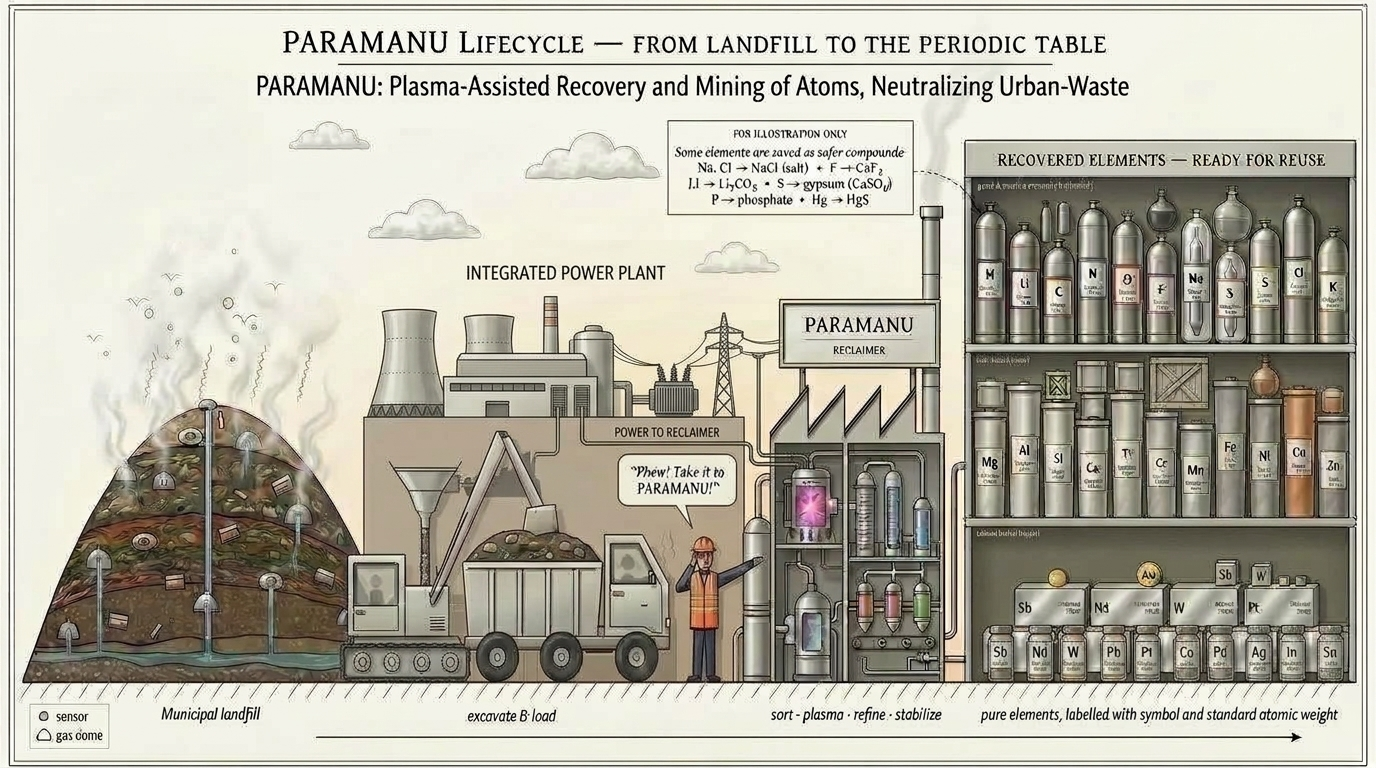
\includegraphics[width=0.85\textwidth]{paramanu_lifecycle_good_with_powerplant.png}
\caption{The PARAMANU lifecycle, from landfill to the periodic table (illustrative artwork; paper Figure 1). An integrated power plant supplies the Reclaimer; recovered elements are stored pure or, where the pure element is reactive or toxic, as safer compounds.}
\end{figure}

\subsection{Landfills as resources}
For two decades researchers have treated landfills as ``anthropogenic resources'' to be mined rather than liabilities to be capped \citep{krook2012,winterstetter2015}. \emph{Enhanced landfill mining} (ELFM) adds energy recovery to material recovery \citep{jones2013}; its reference case is the Remo landfill in Belgium, where characterization found large fine fractions beside recoverable metals and combustibles \citep{quaghebeur2013}. Mining works when the target is simple: one metals-only project in Maine recovered 34,352\,t of ferrous and non-ferrous metals worth about US\$7.42 million \citep{wagner2015}. Case studies and reviews agree that \emph{fines}, the soil-like fraction, dominate mined waste and are the hardest to use \citep{kaartinen2013,hernandez2018,burlakovs2018}; rare earths and platinum-group metals in landfill cores are below ore grade \citep{gutierrez2015}; and the economics are driven by gate fees, energy and material revenues \citep{laner2019}. Every one of these systems separates materials \emph{before} treating them.

\subsection{Plasma treatment of waste}
Thermal plasma, electric arcs at very high temperature, breaks organic material into synthesis gas and melts inorganic residue into glass \citep{heberlein2008,gomez2009}. Plasma gasification of municipal waste makes a hydrogen-rich gas \citep{zhang2012,munir2019} that can drive combined cycles \citep{minutillo2009} or fuel cells \citep{galeno2011}, and plasma gasification with vitrification is a leading waste-to-energy route for ELFM \citep{bosmans2013,danthurebandara2015a}. Vitrified slag leaches little \citep{amutharani2008} and can be used in building products \citep{danthurebandara2015b,machiels2017}. The technology carries real risk: in 2016 Air Products withdrew from its Tees Valley plants, writing down roughly US\$0.9--1.0 billion \citep{icheme2016}. In all these systems plasma \emph{gasifies and melts}; it does not separate elements.

\subsection{Metals spread thin}
Precious metals and rare earths are spread thinly through waste: incinerator bottom ash \citep{morf2013}, fly ash \citep{weibel2021,zucha2020}, even sewage sludge, which in Switzerland carries about 43\,kg of gold and 3,000\,kg of silver per year \citep{vriens2017}. Electronic waste is the richest stream, with established pyro- and hydrometallurgical routes \citep{cui2008,lu2016}. The obstacle is \emph{dilution}: recovery cost rises steeply as concentration falls, the relation first shown by Sherwood \citep{sherwood1959} and confirmed for metals \citep{johnson2007,dahmus2007}; with energy \citep{gutowski2013} and design limits \citep{reck2012}, it explains where recycling stops. This is why 34 of about 60 metals have end-of-life recycling rates below 1\% \citep{graedel2011}.

\subsection{Separating elements after taking material apart}
Three lines of research show that elements can be separated once the material has been taken apart. \emph{Flash Joule heating} vaporizes electronic waste in milliseconds and recovers precious metals by evaporation with less energy than smelting, at laboratory scale \citep{deng2021}. \emph{Plasma mass filters} separate elements by mass in a rotating plasma and have been proposed for nuclear-waste remediation \citep{gueroult2015,zweben2018}. \emph{Microwave hydrogen plasma} treatment of spent lithium-ion battery material enables about 85\% selective lithium recovery in water \citep{chandrasekhar2026}. None treats a whole, mixed waste heap.

\begin{center}
\small
\begin{tabular}{@{}lcccccc@{}}
\toprule
\textbf{Approach} & \textbf{Mixed} & \textbf{Unsorted} & \textbf{Atomic} & \textbf{Sealed,} & \textbf{Element} & \textbf{Toxic} \\
 & \textbf{residue} & \textbf{feed} & \textbf{separation} & \textbf{no stack} & \textbf{bands} & \textbf{capture} \\
\midrule
Landfill mining / ELFM & ∼ & ✗ & ✗ & ✗ & ✗ & ∼ \\
Plasma ELFM & ✓ & ∼ & ✗ & ✗ & ✗ & ✓ \\
Incinerator ash recovery & ✓ & ✗ & ✗ & ✗ & ✗ & ∼ \\
Flash Joule heating & ✗ & ✗ & ✓ & ∼ & ∼ & ✓ \\
Plasma mass filter & ✗ & ✗ & ✓ & ✓ & ∼ & ✗ \\
Fusion torch (1969 concept) & ✓ & ✓ & ✓ & ∼ & ∼ & ∼ \\
\midrule
\textbf{PARAMANU} & ✓ & ✓ & ✓ & ✓ & ✓ & ✓ \\
\bottomrule
\end{tabular}
\end{center}
\noindent Its ingredients exist, and the idea itself is old: in 1968--69 Eastlund and Gough proposed the \emph{fusion torch}, which would use the ultra-hot plasma of a fusion reactor to break any waste into its elements and recover them \citep{eastlund1969}. It stayed a concept, with no design or calculation for real waste. To our knowledge, PARAMANU is the first quantitative, computationally checked design of that idea: a sealed, stack-free reactor with conventional plasma torches that atomizes mixed residual waste and separates its elements by a condensation ladder.

\begin{plain}
Everyone who mines landfills today sorts first, and plasma is used only to burn and melt. The valuable metals are there, but spread so thin that sorting cannot reach them. A few laboratory methods separate elements after vaporizing a material, but none does it for a whole heap of mixed waste. That is the gap PARAMANU aims at.
\end{plain}

%=====================================================================
\section{The Architecture}\label{ch:arch}
%=====================================================================
\subsection{Three stages}
\begin{figure}[H]
\centering
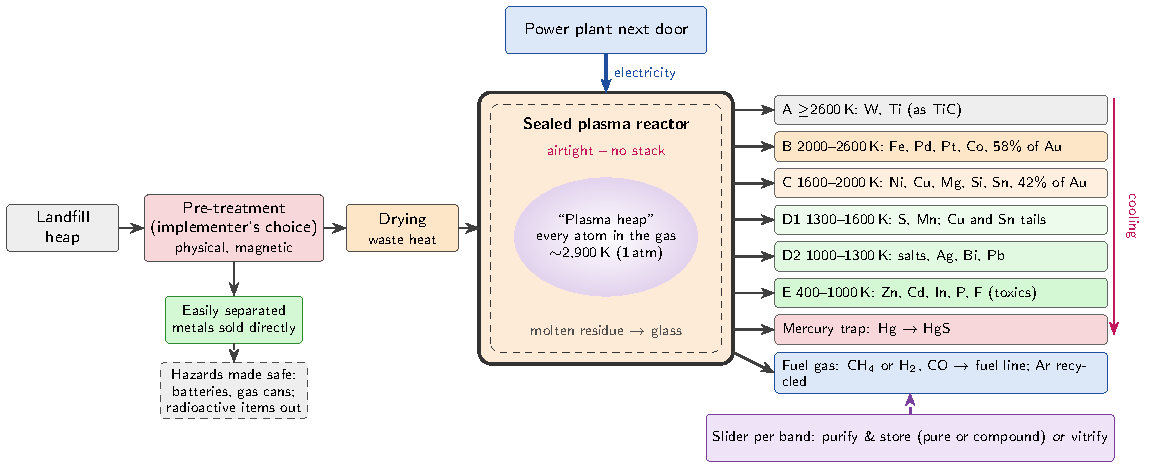
\includegraphics[width=\textwidth]{fig_atomize.pdf}
\caption{The Atomize-First architecture (paper Figure 2).}
\end{figure}

\paragraph{Stage 0: pre-treatment, the implementer's choice.} Existing magnets and eddy currents may remove large pieces of steel and aluminium first. How much, from nothing to a third of the mass or more, is left to the implementer, who knows the feed and the local price of energy. It is encouraged, because each kilogram removed saves about 4\,kWh of plasma energy, but it does not change the quality of the products, which is set by the atomic separation. One part is mandatory: batteries, pressurized cylinders and aerosol cans are discharged, depressurized and dismantled, and anything flagged by radiation portal monitors is removed entirely and handed to a licensed handler. The residue is then dried with waste heat, because water costs energy and adds oxygen.

\paragraph{Stage 1: the sealed plasma hot zone.} The dried residue enters an airtight reactor through an argon-purged lock. Plasma torches heat it until everything is gas. There is no chimney: what a furnace would release as smoke stays inside as part of the heap. The original vision pictured one big sealed batch cooling slowly. The mathematics (Result~5) rules that out, so the reference design keeps the physics but changes the geometry: residue flows continuously or in quick pulses through a sealed train, and each small parcel of gas is its own batch, heated once and cooled once.

\paragraph{Stage 2: atomic separation.} The gas passes condensers held at falling temperatures. Each band is collected, the permanent gases (methane or hydrogen and carbon monoxide, nitrogen) are drawn off to a fuel line (cylinders only at pilot scale), argon is recycled, the molten mineral residue is tapped and made into glass, and each band goes to established refining.

\subsection{The batch cycle, step by step}
The paper states the cycle as an algorithm (for the original batch picture; in the flow design each parcel goes through the same steps in space):
\begin{algorithm}[H]
\caption{Atomize-First cycle for one parcel of residue, from sealed hot zone to separated elements}
\begin{algorithmic}[1]
\Require Pre-treated, dried residue; condenser temperatures $T_{\mathrm{A}} > T_{\mathrm{B}} > T_{\mathrm{C}} > T_{\mathrm{D1}} > T_{\mathrm{D2}} > T_{\mathrm{E}}$ set for the operating pressure from the simulated bands (Result~3); slider $s$
\Ensure Band condensates $\{B_k\}$, trap product, fuel gas, glass; no process gas vented
\State Feed the residue through the argon-purged lock into the sealed train
\State Raise each parcel to the all-gas state in the hot zone, for at most tens of milliseconds \Comment{Result~5}
\For{each band $k = \mathrm{A, B, C, D1, D2, E}$}
  \State Pass the parcel through condenser $k$ held at $T_k$; harvest condensate $B_k$
  \State Filter the fume leaving stage $k$ and return it to $B_k$
  \For{each element $i$ in $B_k$}
    \If{$V_i + s H_i > C_i$} \State send $i$ to purification; store pure or as a stable compound
    \Else \State send $i$ to vitrification \Comment{future ore}
    \EndIf
  \EndFor
\EndFor
\State Capture mercury in the sulfur-impregnated carbon trap; separate the water condensate
\State Compress the remaining gases (CH$_4$, or H$_2$ and CO if quenched; N$_2$) to the fuel line; recycle Ar
\State Tap the molten mineral residue to vitrification; close every element balance over the outlets \Comment{Result~1}
\end{algorithmic}

\end{algorithm}
\noindent Two things in it deserve a note. First, the decision \emph{what to purify} is made per element by the value--harm slider (Chapter~\ref{ch:slider}); what is not purified is not thrown away but vitrified as ``future ore''. Second, the vessel opens only when every outlet is closed: that is the closed-mass principle as an operating rule.

\subsection{The closed-mass principle}
A PARAMANU batch satisfies the \emph{closed-mass principle} if every atom that enters leaves through one of a finite set of labelled outlets (a band collector, a fume filter, a trap, the fuel-gas line, the glass) and none discharges to the atmosphere. The principle governs the process: burning the recovered fuel and generating the electricity have their own stacks, counted in the life-cycle account. This turns ``do we capture the smoke?'' into a design rule: there is no smoke, only product streams not yet harvested. It is also the first acceptance test of a real plant (Result~1).

\subsection{Storing what is recovered}
The rule: store the pure element when it is stable in air and water and sold that way; otherwise store a stable compound.
\begin{center}
\small
\begin{tabular}{@{}>{\raggedright\arraybackslash}p{3.3cm}>{\raggedright\arraybackslash}p{5.6cm}>{\raggedright\arraybackslash}p{5.4cm}@{}}
\toprule
\textbf{Form} & \textbf{Elements} & \textbf{Stored as} \\
\midrule
Pure metal & Fe, Al, Cu, Zn, Pb, Ni, Co, Sn, Bi, In, Ga, Mg (alloy) & ingots, cathodes, alloy \\
Pure precious metal & Au, Ag, Pd, Pt, Rh & bullion, sponge \\
Pure non-metal & H, S, C, Se, Te & H\textsubscript{2} cylinders, sulfur blocks, carbon black \\
Compound (reactive) & Li, Na, K, Ca & Li\textsubscript{2}CO\textsubscript{3}, NaCl, KCl, CaSO\textsubscript{4} \\
Compound (hazardous gas) & F, Cl, N, P & CaF\textsubscript{2}, NaCl, ammonium sulfate, phosphate \\
Compound (toxic) & Hg, Cd, As, Cr & HgS, CdS, scorodite, Cr\textsubscript{2}O\textsubscript{3} \\
Oxide & rare earths, Mn, V, Sb, W & oxides, tungsten carbide \\
\bottomrule
\end{tabular}
\end{center}
Why these forms: the reactive alkali metals would burn or react with water if stored pure; the halogens and nitrogen are gases or corrosive; the toxic elements are stored in the forms nature itself has kept stable for geological time (Chapter~\ref{ch:landfill}).

\begin{plain}
Sort only what is easy and dangerous; seal the rest in a box with no chimney; heat it briefly to gas; cool it past a row of collectors; bottle the gas; turn the leftover minerals into glass.
\end{plain}

%=====================================================================
\section{The Condensation Ladder}\label{ch:ladder}
%=====================================================================
\subsection{A first guide: boiling points}
\begin{center}
\small
\begin{tabular}{@{}ll>{\raggedright\arraybackslash}p{9.6cm}@{}}
\toprule
\textbf{Band} & \textbf{Range} & \textbf{Elements (normal boiling point, K)} \\
\midrule
I & $>$3,500\,K & W 5828, Ta 5731, Mo 4912, Zr 4682, Pt 4098, C 3915 (sublimes), V 3680, Ti 3560, Si 3538 \\
II & 2,800--3,500\,K & Nd 3347, Pd 3236, Co 3200, Ni 3186, Fe 3134, Au 3129, Cr 2944, Sn 2875, Cu 2835 \\
III & 2,000--2,800\,K & Al 2743, Ga 2673, Ag 2435, In 2345, Mn 2334, Ba 2170, Pb 2022 \\
IV & 1,000--2,000\,K & Sb 1860, Bi 1837, Ca 1757, Sr 1655, Li 1615, Mg 1363, Zn 1180, Na 1156, Cd 1040, K 1032 \\
V & $<$1,000\,K & Se 958, As 887 (sublimes), S 718, Hg 630, P 553 \\
Gases & -- & H\textsubscript{2}, CO, N\textsubscript{2} (to a fuel line); Ar (recycled) \\
\bottomrule
\end{tabular}
\end{center}
\begin{figure}[H]
\centering
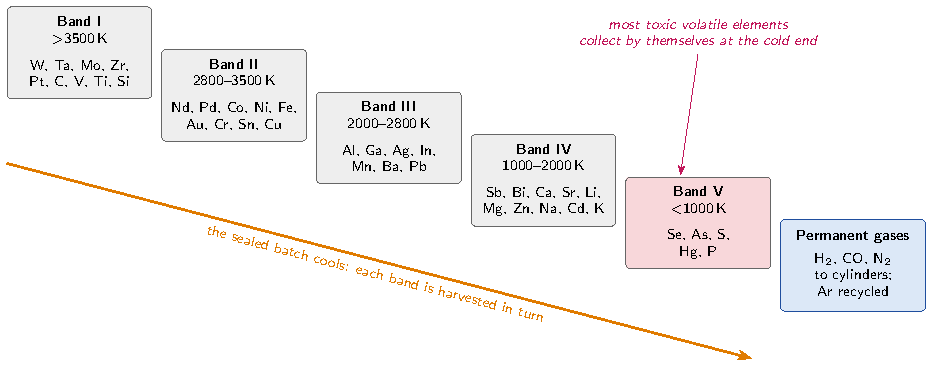
\includegraphics{fig_ladder.pdf}
\caption{The condensation ladder as first conceived: as the sealed batch cools, each band is harvested in turn.}
\end{figure}

The first version of the idea grouped elements by their normal boiling points into five bands I--V (tungsten at 5,828\,K down to phosphorus at 553\,K; paper Table~2). This is only a guide, for three reasons the simulation later made precise:
\begin{itemize}
\item \textbf{Dilute elements condense far below their boiling points.} An element that is 1\% of the gas does not condense until its vapor pressure falls to 1\% of the total pressure, hundreds of kelvin lower (Result~3).
\item \textbf{Elements are not alone.} Oxygen, chlorine and fluorine form oxides and salts with their own volatility; metals dissolve in one another.
\item \textbf{Neighbours co-condense.} Iron, nickel, cobalt, copper and gold condense close together, so a band is an alloy, not a pure element, and final purification uses established refining.
\end{itemize}

\subsection{The simulated ladder}
The simulation replaced the guide with an equilibrium calculation of the whole heap (Chapter~\ref{ch:results}). At 1\,atm the first solid appears at 2,875\,K; nothing condenses above 3,500\,K, because the heap is a dilute molecular gas (CO, H\textsubscript{2}, SiO). The bands it suggests are:

\begin{center}
\small
\begin{tabular}{@{}l l >{\raggedright\arraybackslash}p{8.2cm} r@{}}
\toprule
\textbf{Band} & \textbf{Range (K)} & \textbf{Main elements collected (default feed, 1\,atm)} & \textbf{kg/t} \\
\midrule
A & $\ge$2,600 & W, Ti (as TiC); part of Si and Nd & 20.7 \\
B & 2,000--2,600 & Fe (metal), Pd, Pt, Co, 58\% of the Au, Nd; Al and Ca as oxides & 140.2 \\
C & 1,600--2,000 & Mg, Si, Ni, Cu, Cr, Sn, Sb, Ga, 42\% of the Au & 171.5 \\
D1 & 1,300--1,600 & S, Mn; tails of Cu, Sn, Sb, Cr, Ga; in organic-rich feeds, gold that passes Band C & 4.1 \\
D2 & 1,000--1,300 & Na, K, Cl (as salts), Ag, Bi, most of the Pb & 85.8 \\
E & 400--1,000 & Zn, Cd, In, Li, F, P, the rest of the Pb; carbon & 61.8 \\
Cold & $<$400 & water, carbon & 208.1 \\
Gas & -- & CH\textsubscript{4} (at equilibrium), N\textsubscript{2}; about half of the Hg & 19.4 \\
\bottomrule
\end{tabular}
\end{center}

Band D was originally one band, 1,000--1,600\,K. It was split into D1 and D2 after the adversarial search found feeds in which gold and lead shared it (Section~\ref{sec:adversary}).

\subsection{The heap carries its own reducing agent}
If oxygen recombined with the metals during cooling, the bands would hold oxides, not metals. The waste supplies the remedy: its plastics and paper are rich in carbon and hydrogen, which bind oxygen as CO and water. With simple proxies (silica for soil and glass, polyethylene for plastics, cellulose for paper), one wet tonne holds about 18,300\,mol of oxygen, 13,000\,mol of carbon and 24,800\,mol of hydrogen, so the ratio
\[
\frac{n_{\mathrm C} + n_{\mathrm H}/2}{n_{\mathrm O}} = \frac{12{,}955 + 24{,}799/2}{18{,}254}\approx 1.39
\]
exceeds one: there is 1.4 times the reductant needed. With the full feed model the ratio is 1.52, and the equilibrium calculation confirms it: iron condenses 100\% as metal, against 43\% if the organics are removed (Section~\ref{sec:reductant}).

\begin{plain}
Things do not come out at their textbook boiling points; they come out much cooler, and in groups. The groups (bands) are set by calculation, not by a table. And the plastic in the trash is useful: it keeps the metals from rusting as they condense.
\end{plain}

%=====================================================================
\section{The Mathematics: Eight Results}\label{ch:math}
%=====================================================================
Mathematics cannot prove that a plant works; materials, kinetics and engineering decide that. It can prove what physics permits and forbids, and turn those limits into design equations. \textbf{None of this mathematics is new}: the eight results are standard consequences of thermodynamics and convex optimization (conservation of mass; Gibbs-energy minimization \citep{gordon1994,boyd2004}; Clausius--Clapeyron; the Fenske equation of distillation; grey-body radiation with the isoperimetric inequality; the ideal entropy of mixing; detailed balance). What is new is their application to atomic recovery from waste, where each becomes a design rule, a sizing number or an acceptance test. The paper gives eight such results with proofs. For each, this chapter gives the statement, why it is true, what it is used for, and how it was checked.

Notation: $T$ temperature, $P$ pressure, $P_0 = 1$\,atm, $R$ the gas constant, $n_i$ the moles of element $i$, $a_k$ the vector of atoms in species $k$, and $g_k = G^\circ_k/RT$.

\subsection{Result 1: Every atom is accounted for}
\textbf{Statement.} If the closed-mass principle holds, for every element $i$ the moles entering equal the sum over all outlets: $\sum_{o} n_{i,o} = n_i^{\mathrm{in}}$.

\textbf{Why.} Chemistry rearranges atoms but never creates or destroys them, and with no path to the air every atom that leaves goes through a labelled outlet.

\textbf{Use.} The first acceptance test of any plant: measured outlets must close every element balance within measurement error. In the simulation every element above one part per million of the gas balances to better than $10^{-4}$ at every step, and the certificate (Chapter~\ref{ch:verification}) checks this for every state.

\paragraph{Worked example: what has to balance.} For the default feed (one wet tonne, 5.2\% pre-treatment) the batch holds the element amounts below. Result~1 says each row must reappear, summed over all outlets, at the end. In the simulation this is checked at every step and for every state by the certificate.
\input{tables/feed_elements}

\subsection{Result 2: The equilibrium exists and is unique}
\textbf{Statement.} For an ideal gas with any number of pure condensed phases and ideal solutions at fixed $T$ and $P$, the minimum Gibbs energy subject to the element balances exists; the composition of the gas and of each solution there is unique; and the element potentials $\lambda$ solve the concave dual problem
\[
\max_{\lambda} \sum_i n_i\lambda_i \ \text{ s.t. } \sum_{k\in\text{gas}} e^{a_k\cdot\lambda - g_k - \ln(P/P_0)}\le 1,\ \ \sum_{k\in s} e^{a_k\cdot\lambda - g_k}\le 1,\ \ a_c\cdot\lambda\le g_c .
\]
\textbf{Why.} The allowed compositions form a closed, bounded set, so a minimum exists. The Gibbs energy of each mixture is strictly convex in its mole fractions, so they are unique. The constraints are linear, so convex duality holds, and the multipliers are the element potentials. At the optimum every species present obeys $\ln x_k = a_k\cdot\lambda - g_k$ ($-\ln(P/P_0)$ in the gas), and a pure phase exists only where $a_c\cdot\lambda = g_c$.

\textbf{Use.} (i) The answer of the solver is \emph{the} equilibrium, not one of several. (ii) The state entering the condensers depends only on the feed's element totals, $T$ and $P$, not on how the torches got there. (iii) The same conditions give the \emph{certificate} that checks any computed state (Chapter~\ref{ch:verification}).

\paragraph{Why the dual matters: element potentials as prices.} A useful way to read Result~2: each element $i$ gets one ``price'' $\lambda_i$. A species' mole fraction is set by the total price of its atoms minus its own Gibbs energy: $\ln x_k = a_k\cdot\lambda - g_k$. A solid or liquid forms only when the price of its atoms reaches its Gibbs energy ($a_c\cdot\lambda = g_c$); if the atoms are ``cheaper'' than that, it stays absent. Finding the equilibrium is then finding one price per element, a handful of numbers, instead of hundreds of species amounts. That is why the solver works in the dual, why the dilute-limit solver needs only one new price per trace, and why the certificate can check any state by fitting the prices back.

\paragraph{How the solver uses it, step by step.}
\begin{enumerate}
\item Gas only: CEA Newton iteration on the gas amounts and the multipliers of the element balances.
\item If some condensed phase would be supersaturated ($a_c\cdot\lambda > g_c$), solve the dual problem above for $\lambda$ with a constrained optimizer.
\item Read off the active phases (those with $a_c\cdot\lambda \approx g_c$) and compute their amounts from the element balances by non-negative least squares.
\item Polish: a CEA Newton iteration with the phase set fixed, to full precision.
\item Certify (Chapter~\ref{ch:verification}); if a phase was missed, add it and repeat (the CEA phase-set loop).
\end{enumerate}

\subsection{Result 3: When a dilute element condenses}
\textbf{Statement.} An element at gas mole fraction $y$ begins to condense as a pure phase where $yP = p^{\mathrm{sat}}(T_c)$; approximately
\[
\frac{1}{T_c} = \frac{1}{T_b} - \frac{R}{\Delta H_{\mathrm{vap}}}\ln\frac{yP}{P_0}.
\]
If it dissolves in a condensing host with activity coefficient $\gamma$ at mole fraction $x$, the condition is $yP = \gamma x\, p^{\mathrm{sat}}$.

\textbf{Why.} Condensation begins when the element's chemical potential in the gas equals that in the condensed phase; integrating the Clausius--Clapeyron equation from the boiling point gives the closed form.

\textbf{Use.} It explains why the simulated ladder sits hundreds of kelvin below boiling points, why every band moves with pressure (through $yP$), and why mercury, at about 2\,ppm, never reaches saturation at 1\,atm. \textbf{Checked:} closed form, exact condition and full simulation agree (Fe 2,315 / 2,330 / 2,320\,K; Ni 1,882 / 1,905 / 1,900; Cu 1,760 / 1,774 / 1,770; Pb 1,061 / 1,070 / 1,070; Zn 715 / 722 / 720), within 18\,K.

\paragraph{Worked example: iron.} In the default heap at the start of condensation, iron is $y = 0.008524$ of the gas at $P = 1$\,atm; its normal boiling point in the data is $T_b = 3{,}139$\,K and $\Delta H_{\mathrm{vap}} = 349.2$\,kJ/mol. Then
\[
\frac{1}{T_c} = \frac{1}{3139} - \frac{8.314}{349{,}200}\ln(0.008524) = 3.186\times10^{-4} + 2.381\times10^{-5}\times 4.765 = 4.320\times10^{-4},
\]
so $T_c = 2{,}315$\,K, 824\,K below the boiling point. The exact condition gives 2,330\,K and the full simulation 2,320\,K. The same calculation for each metal:
\input{tables/theory_onset}
\paragraph{Why the bands move with pressure.} $yP$ is the controlling quantity. At 5\,atm every $yP$ is five times larger, so every element condenses hotter; at 0.1\,atm ten times smaller, so colder. This is exactly what the sweep shows: gold's half-condensation temperature has a median of 1,700\,K at 0.1\,atm, 2,100\,K at 1\,atm and 2,350\,K at 5\,atm. It also explains mercury: at about 2\,ppm of the feed its $yP$ is so small that at 1\,atm it reaches saturation only near room temperature, so half of it is still gas at 300\,K.

\subsection{Result 4: Which elements physics can separate}
\textbf{Statement.} For two elements with relative volatility $\alpha>1$: a single condensation leaves $(1-f)^{1/\alpha}$ of the lighter element in the gas when a fraction $f$ of the heavier one has condensed; and a split to purity $p$ needs at least $N_{\min} = \ln[p^2/(1-p)^2]/\ln\alpha$ ideal stages (the Fenske equation of distillation).

\textbf{Use.} It says what the ladder can and cannot do. With NASA vapor pressures: zinc, magnesium and mercury leave iron or zinc in one stage; lead from copper in 1.5; silver from gold in about 2; copper from nickel in 3.5; cadmium from zinc in 5. But gold from iron ($\alpha = 1.43$) needs 26 stages, palladium from iron 22, nickel from cobalt 69, tin from copper 258. \textbf{Physics separates the toxic volatile metals from the precious ones; it does not separate gold or palladium from iron.} Those leave the iron band by established refining. The paper states this plainly.

\paragraph{Worked example: gold and iron.} With $\alpha = 1.43$ and a 99\%/99\% split, $N_{\min} = \ln(0.99^2/0.01^2)/\ln 1.43 = \ln 9801/0.358 = 9.19/0.358 = 25.7$, so 26 ideal stages. By contrast zinc against iron at 1,500\,K has $\alpha \approx 8\times10^{7}$: when 99\% of the iron has condensed, the fraction of zinc left in the gas is $(0.01)^{1/\alpha} \approx 1$; essentially all the zinc is still gaseous, and one stage suffices. The full table:
\input{tables/theory_volatility}
\begin{figure}[H]
\centering
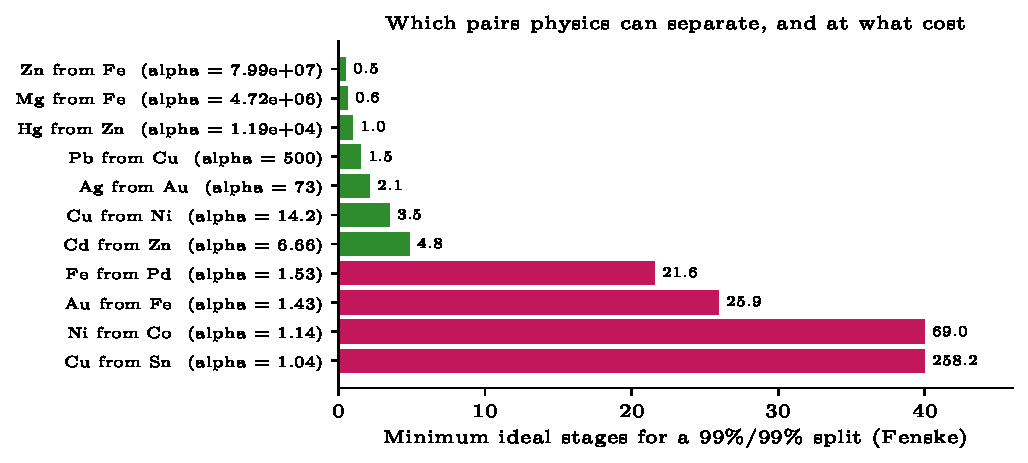
\includegraphics[width=0.9\textwidth]{fig_fenske.pdf}
\caption{Minimum ideal stages for a 99\%/99\% split of key pairs (bars capped at 40).}
\end{figure}

\subsection{Result 5: How briefly the heap must be hot}
\textbf{Statement.} A batch of mass $m$ that needs specific energy $e$ and forms $\nu$ moles of gas per kilogram, radiating to walls at $T_w$ with emissivity $\varepsilon$, loses its own energy in
\[
\tau = \frac{e\,m}{\varepsilon\sigma(36\pi)^{1/3}(\nu mRT/P)^{2/3}(T^4-T_w^4)} \propto m^{1/3}P^{2/3},
\]
and a continuous hot zone with residence time $t_r$ loses the fraction $Q/\dot W \propto t_r^{2/3}\dot m^{-1/3}$ of its torch power. A sphere is the best case, so any real vessel does worse.

\textbf{Why.} Ideal-gas volume, the isoperimetric inequality (a sphere has the least surface for its volume) and grey-body radiation.

\textbf{Use.} This is the result that changed the design. A one-tonne batch at 2,890\,K radiates its own energy in about 4.2\,s (the simulation reproduces the $m^{1/3}$ law with exponent 0.333), so a slowly cooling sealed batch is impossible at any size. A continuous or pulsed hot zone at 1,000 tonnes per day keeps radiation below 10\% of torch power if each parcel stays at most 25\,ms (below 5\% at 10\,ms). Larger plants are easier, because the loss falls as $\dot m^{-1/3}$.

\begin{figure}[H]
\centering
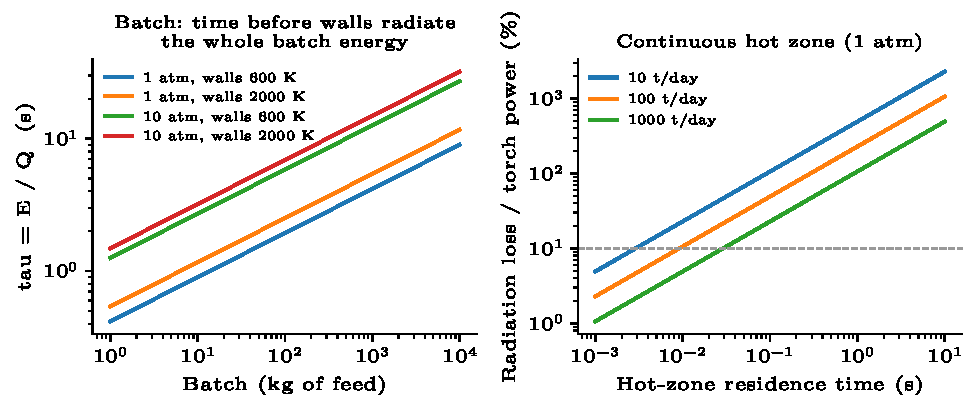
\includegraphics[width=\textwidth]{fig_reactor_design.pdf}
\caption{Result 5: radiation time constant of a sealed batch (left) and radiation loss of a continuous hot zone against residence time (right).}
\end{figure}

\paragraph{Worked example: the reference plant.} At 1,000 tonnes of excavated material per day the feed is $\dot m = 11.57$\,kg/s; at 2,890\,K and 1\,atm it makes 35.1\,mol of gas per kg, 96\,m\textsuperscript{3}/s. For 5\% radiation loss the residence time is 10\,ms, the hot volume 1.0\,m\textsuperscript{3} and the torch power 119\,MW; for 10\% loss, 25\,ms, 2.4\,m\textsuperscript{3} and 126\,MW (with $e = 9.8$\,MJ per kg of excavated material, drying excluded because it uses waste heat). The batch time constant and the loss of a continuous hot zone, from the simulation:
\begin{center}
\begin{minipage}[t]{0.38\textwidth}\centering\textbf{Sealed batch, 1\,atm, walls 600\,K}\\[3pt]\input{tables/batch_tau}\end{minipage}\hfill
\begin{minipage}[t]{0.6\textwidth}\centering\textbf{Continuous hot zone: radiation loss (\% of torch power), 1\,atm}\\[3pt]\input{tables/flow_loss}\end{minipage}
\end{center}
A tonne-size batch loses its energy in seconds, while a millisecond flow at plant scale loses a few per cent: that single comparison is why the reactor is a flow, not a slowly cooling batch.

\subsection{Result 6: Separation itself is cheap}
\textbf{Statement.} Unmixing an ideal mixture into pure elements at $T_0$ needs at least $W_{\min} = -RT_0\sum_i n_i\ln x_i$.

\textbf{Use.} For the default feed $W_{\min} = 0.067$\,MWh per tonne, only 2.3\% of the energy needed to reach the all-gas state. The energy goes into vaporizing and into the walls, not into separating. Efficiency work therefore belongs in shorter hot zones and heat recovery.

\paragraph{Worked example.} The default heap needs 2.9\,MWh per tonne to become gas; unmixing it into pure elements needs at least $W_{\min} = 0.067$\,MWh, so $0.067/2.9 = 2.3\%$. Even a separation process ten times less efficient than the ideal would spend less on separating than on vaporizing.

\subsection{Result 7: The heap forgets what it was}
\textbf{Statement.} At fixed $T$ and $P$ the equilibrium of a closed batch depends on the feed only through its element totals. Any two feeds with the same atoms, whatever molecules they were, reach the same equilibrium.

\textbf{Why.} Neither the Gibbs energy nor the constraints mention the original molecules; the feed enters only through the element totals, and Result~2 makes the minimum unique.

\textbf{Use.} This is why household, industrial and medical waste, with its polymers, pharmaceuticals, PFAS and solvents, needs no molecule-by-molecule treatment: sorting by molecule is replaced by accounting by element. \textbf{Checked} two ways (script \texttt{13\_breakdown.py}): three very different starting mixtures with identical atoms (bare atoms; aromatics with CF\textsubscript{4}, CCl\textsubscript{4}, phosgene and chloromethane; monomer-like molecules) reach the same state to $10^{-11}$ in Cantera and $3\times10^{-9}$ in PARAMANU; and in the real heap at 2,890\,K the equilibrium mole fractions of those starting molecules are vanishing: naphthalene $10^{-28}$, benzene $10^{-18}$, CCl\textsubscript{4} $10^{-26}$, phosgene $10^{-16}$, CF\textsubscript{4} $10^{-39}$.

\paragraph{The data behind the checks.} Equilibrium mole fractions of complex molecules in the real heap at several temperatures (default feed, all phases):
\input{tables/breakdown_molecules}
Three starting mixtures with identical atoms reach the same state; the largest relative difference of any major species against the atoms-only start, at each temperature:
\input{tables/breakdown_starts}

\subsection{Result 8: A catalyst cannot change the outcome}
\textbf{Statement.} A catalyst that is not consumed changes no equilibrium constant, and so does not change the equilibrium of the heap at any temperature or pressure; a catalyst that does not survive becomes part of the feed and acts only through the atoms it adds.

\textbf{Why.} $K = e^{-\Delta_r G^\circ/RT}$ depends only on reactants and products. In transition-state theory a catalyst lowers the barrier for the forward and the reverse reaction by the same factor, so $k_f/k_r = K$ is unchanged (detailed balance). Result~2 then fixes the state.

\textbf{Use.} A catalyst can only change \emph{how fast} the heap reaches its equilibrium, which matters only where the reaction would otherwise be too slow (Chapter~\ref{ch:catalysts}).

\paragraph{The data behind the check.} Lifetime of CF\textsubscript{4}, the hardest molecule to break, and the Damk\"ohler number of a 25\,ms hot zone:
\input{tables/cat_damkohler}
Where Da is in the hundreds, the reaction is long finished before the gas leaves; a catalyst could only matter where Da is near or below one.

\begin{wherecode}
Proofs worked through with exercises: \texttt{docs/STUDENT\_GUIDE.md}. Numerical checks: \texttt{scripts/07\_theory\_checks.py} (Results 3, 4, 6), \texttt{08\_reactor\_design.py} (Result 5), \texttt{13\_breakdown.py} (Result 7), \texttt{17\_catalysts.py} (Result 8). Closed-form theory in code: \texttt{paramanu\_sim/theory.py}. Tests: \texttt{tests/test\_theory.py}.
\end{wherecode}

%=====================================================================
\section{The Chamber at Work: Hardware Tied to Proof}\label{ch:walk}
%=====================================================================
The paper follows one parcel of residue through a reference plant, treating 1,000 tonnes of excavated material per day at 1\,atm, and names at each station the result that governs it, the number it sets, and the measurement that would verify it.

\begin{figure}[H]
\centering
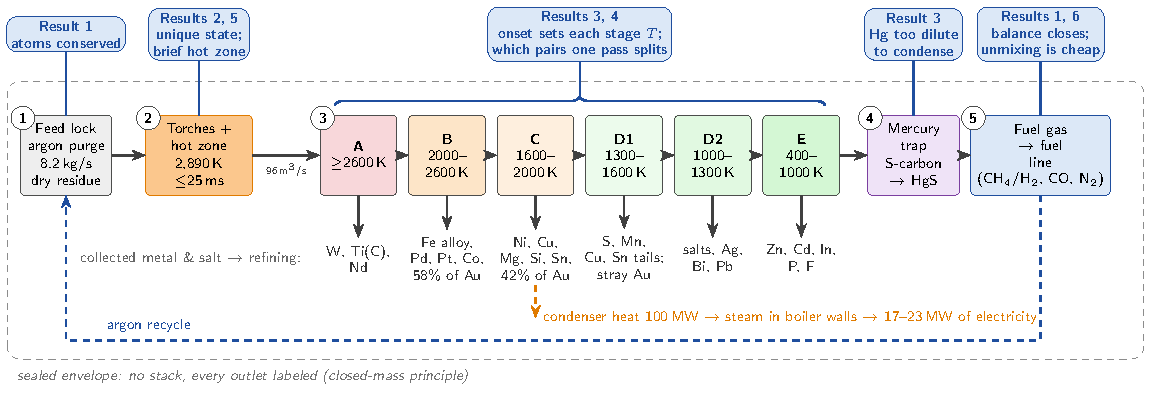
\includegraphics[width=\textwidth]{fig_chamber.pdf}
\caption{The reference plant and the result governing each station (paper Figure 8).}
\end{figure}

\paragraph{A batch in time equals a flow in space.} Each parcel of gas flowing through the sealed train is heated once and cooled once, and meets the condensers in order of falling temperature. A parcel that passes the stage at temperature $T$ undergoes exactly one step of the simulated ladder. So the ladder in time and the train in space are the same calculation, provided three measurable conditions hold: \textbf{plug flow} (parcels do not mix back; measured with a tracer pulse), \textbf{equilibrium in each stage} (measured by the gas composition at each stage exit against Result~3), and \textbf{condensate stays out} (measured by each collector's element balance against Result~1).

\begin{center}
\small
\begin{tabular}{@{}>{\raggedright\arraybackslash}p{2.3cm}>{\raggedright\arraybackslash}p{1.3cm}>{\raggedright\arraybackslash}p{5.6cm}>{\raggedright\arraybackslash}p{5.2cm}@{}}
\toprule
\textbf{Station} & \textbf{Result} & \textbf{Design number (1,000\,t/day, 1\,atm)} & \textbf{Verified by measuring} \\
\midrule
1 Feed lock & 1 & 11.6\,kg/s excavated, 8.2\,kg/s dry residue through an argon-purged lock; no outlet to air & every element balance closes over the outlets \\
2 Hot zone & 2, 5 & 2,890\,K; at least 113\,MW (121\,MW with drying; about 280\,MW at the best demonstrated specific energy); 35.1\,mol gas per kg, 96\,m\textsuperscript{3}/s; $\le$25\,ms, 2.4\,m\textsuperscript{3} (a sphere 1.7\,m across) & exit-gas composition against equilibrium; wall heat flux against Result~5 \\
3 Condensers & 3, 4 & six stages A, B, C, D1, D2, E; duties 13.6, 28.3, 21.9, 3.3, 11.5 and 15.7\,MW (100\,MW with the cold end, 42\% above 2,000\,K); 0.24, 1.62, 1.99, 0.05, 0.99 and 0.72\,kg/s collected & onset temperature of each element against Result~3; purity of each band against Result~4 \\
4 Mercury trap & 3 & a median 58\% of the mercury reaches it at 1\,atm (10\% at 5\,atm, all at 0.1\,atm): sulfur-impregnated carbon, product HgS & mercury in the trap against the bands \\
5 Gas store & 1, 6 & 13.7\,mol/s of CH\textsubscript{4} (or H\textsubscript{2} and CO if quenched fast) with N\textsubscript{2}; argon recycled & gas composition; C, H and N balances \\
\bottomrule
\end{tabular}
\end{center}

%=====================================================================
\section{Why the Chamber Does Not Melt}\label{ch:walls}
%=====================================================================
A gas at 2,890\,K is hotter than the melting point of steel (about 1,800\,K), copper (1,358\,K) and almost every refractory; the chamber survives because no wall ever has to be as hot as the gas. The paper (Section ``Why the Chamber Does Not Melt'') gives four reasons the chamber survives, each already used in high-temperature industry, and each with a number a pilot must confirm.
\begin{enumerate}
\item \textbf{The walls see heat, not plasma.} The arcs attach only to electrodes or to the molten bath. The wall receives radiation and the heat of the passing gas. With the grey-gas model ($\varepsilon = 0.3$, walls at 600\,K) the radiative flux is $q = 0.3\times5.67\times10^{-8}\times(2{,}889^4 - 600^4) \approx 1.2$\,MW\,m\textsuperscript{-2}; on the 8.7\,m\textsuperscript{2} wall of the reference hot zone (2.4\,m\textsuperscript{3}, 1.7\,m across) that is about 10\,MW, 9\% of the 113\,MW torch power. Water-cooled metal walls remove fluxes of this order routinely; rocket combustion chambers handle one to two orders of magnitude more. Convection from gas moving at about 44\,m/s adds to it and must be measured.
\item \textbf{The hot face is made of the process's own material.} On a water-cooled copper wall, molten residue or condensate freezes into a solid \emph{skull} whose hot face sits at its own melting point; it insulates the metal and heals itself. Each stage is lined with its \emph{own} product so the lining cannot contaminate the band: in the hot zone the molten residue itself (anything condensing there rejoins the feed and is vaporized again, losing nothing by Results~1 and~7), and in each condenser that band's own condensate, collected by a shower of its own liquid as lead splash condensers capture zinc in zinc smelting. Where a refractory is used, the reducing, oxygen-poor gas allows carbon and carbides. Where a refractory is used instead, the heap's reducing, oxygen-free gas allows graphite and carbides, which would burn in air (graphite sublimes near 3,900\,K).
\item \textbf{The hot gas is kept off the walls by flow, not by fields.} Magnets cannot hold the heap: a field acts only on charged particles, and at 2,890\,K only about 1 particle in 5,000 is charged. Even a fully ionized gas at 1\,atm would need $B \ge \sqrt{2\mu_0 P} \approx 0.5$\,T over the whole chamber just to balance its pressure. So the gas \emph{flows}: a swirling core and a curtain of cooler gas along or through the wall, as induction plasma torches use a sheath gas, keep the hottest gas away from the wall. The curtain dilutes the heap; the model shows argon equal to half or all of the heap's gas lowers every condensation temperature by 25--150\,K and shifts gold toward the copper band (58\% $\to$ 50\% and 44\% in Band B), while zinc and lead still stay out of the gold bands and all the mercury stays gaseous for the trap. Recycling the process's own cleaned gas as the curtain avoids a foreign gas.
\item \textbf{Brevity makes it manageable.} Result~5 already requires a small, brief hot zone: a few square metres of hot wall per 1,000 tonnes per day, and milliseconds of contact. Downstream, each stage's wall need only stand its own band's temperature.
\end{enumerate}
\textbf{What must be demonstrated} (research question R4, on a bench reactor of a few tens of kilowatts first): that a skull of the right composition forms and stays stable in each stage; that walls do not collect another band's condensate; that the gas curtain keeps the wall flux near 1\,MW\,m\textsuperscript{-2}; and that convective and radiative loads match the estimate.

%=====================================================================
\section{Fume: The Largest Open Risk}\label{ch:fume}
%=====================================================================
Every separation result assumes equilibrium: what condenses at a stage stays at that stage. Rapid cooling can break this. Metal and oxide vapor quenched in milliseconds nucleates into \emph{fume}, particles of a fraction of a micrometre that ride the gas instead of settling on the condenser, and traces such as gold can condense onto them and travel with them.
\begin{itemize}
\item \textbf{Industry knows it.} The SiO that leaves silicon and ferrosilicon furnaces becomes silica fume of 0.1--0.5\,\textmu m particles, caught in bag filters and sold for concrete \citep{aci234r06}. SiO is a main species of the PARAMANU heap, so fume is certain; the open question is how much of each element it carries past its band.
\item \textbf{The design answer.} A fume filter after every stage (an electrostatic precipitator or a hot ceramic filter) returns its catch to that stage's collector, and each stage holds the gas long enough for growth on the condensate, rather than in the gas, to dominate. Off-band catch can also be recycled to the feed, which by Results 1 and 7 loses nothing.
\item \textbf{The test.} Measuring the fume that reaches each band is the first task of research questions R1 and R2, and it decides predictions P5--P9. This is why the paper names fume first among the effects the model leaves out.
\end{itemize}

%=====================================================================
\section{Practical Answers to Five Engineering Objections}\label{ch:practical}
%=====================================================================
Five objections follow naturally from the numbers above. Each has an answer that industry already uses, quantified here with script \texttt{24\_heat\_recovery\_and\_scale.py}.

\textbf{``No heat engine works at 2,000\,K.''} None has to. The condenser stages are built as the radiant water walls of a steam boiler. Coal-fired boiler walls already face flames near 1,900\,K, and the evaporative cooling systems and waste-heat boilers of electric arc furnaces take off-gas from about 1,700\,\textdegree C down to 200\,\textdegree C and turn its heat into steam \citep{gandt2016}. The same water-cooled wall carries each stage's protective skull. If 60--70\% of the stage heat is captured as steam and a steam cycle converts it at 30--35\%, the 2.26\,MWh per tonne released in stages A--E yields \textbf{0.41--0.55\,MWh of electricity per tonne}, or 17--23\,MW for 1,000 tonnes per day. The exergy of the hottest heat is not fully used, but the energy is not thrown away.

\textbf{``The emissivity is optimistic.''} Gas carrying condensing particles can radiate nearly as a black body. At the 25\,ms design point the hot zone loses 9\% of its power at $\varepsilon = 0.3$, but 18\% at $\varepsilon = 0.6$ and 30\% at $\varepsilon = 1$; keeping the loss below 10\% then needs about 10 and 5\,ms, and the wall flux rises from 1.2 to 3.9\,MW\,m\textsuperscript{-2}. The design can take either route: shorten the residence time, or accept the loss, because radiation that reaches a boiler wall becomes steam rather than waste.

\textbf{``No one can build a 113--280\,MW hot zone.''} The plant does not have to be one unit. Split into parallel modules, 1,000 tonnes per day becomes 2--10 trains of 11--130\,MW each, the scale of existing arc furnaces. Smaller modules lose relatively more to radiation ($\dot m^{-1/3}$): ten modules of 100 tonnes per day need 9\,ms for 10\% loss at $\varepsilon = 0.3$, but only 1.5\,ms at $\varepsilon = 1$. The best choice is therefore a few large modules, two to four, rather than many small ones.

\textbf{``Nobody can grind landfill to 20\,\textmu m.''} Only the mineral fraction needs it. The organics crack to gas below about 500\,\textdegree C (Chapter~\ref{ch:results}), so the residue is first dried and pyrolyzed; what remains is a brittle mineral char. A cement-plant vertical roller mill grinds raw meal for about 19\,kWh/t \citep{jca_vrm}, and scaling to 20\,\textmu m by Bond's law gives about \textbf{29\,kWh per tonne of waste, 1\% of the plasma energy}. Oversize goes to the molten bath of a transferred-arc furnace instead of the powder stream.

\textbf{``The bands are slag, not metal.''} Most of each band's mass is oxide, and that is exactly how precious-metal smelting works. Each collector is a settling hearth in which the liquid metal sinks under the lighter slag and the two are tapped separately. Band B is an \emph{iron collector}: plasma smelting of spent car catalysts with iron as the collector is the industrial route at Johnson Matthey and Heraeus, and it recovers 99.3\% of the palladium, 99.1\% of the platinum and 97.2\% of the rhodium into an iron alloy while the oxides leave as slag \citep{liu2026pgm}. The slag of each band then joins the mineral products or the glass.


%=====================================================================
\section{How the Simulation Works}\label{ch:code}
%=====================================================================
The simulation is open Python code in the \texttt{simulation} folder. This chapter explains what it does, step by step, so that a reader can follow any number back to its origin.

\subsection{The feed: one wet tonne as elements}
One wet tonne of excavated landfill material is modelled as 250\,kg of water and 750\,kg of dry components (before pre-treatment): fines (soil) 375\,kg, plastics 135, paper and wood 90, glass 90, ferrous metal 30, other residue 18.4, non-ferrous metal 9, electronic waste 2.25 and batteries 0.375\,kg; the masses come from the Sort-First baseline spreadsheet. Each component has a proxy composition:
\begin{itemize}
\item \textbf{Fines}: the oxides of the upper continental crust \citep{rudnick2003}, 10\% cellulose, 1\% protein-like nitrogen, 1\% gypsum, and the heavy metals measured in landfill fines by \citet{vollprecht2020} (mean of four size classes: copper 383, zinc 996, lead 729, chromium 81 and nickel 70\,mg/kg) as oxides. Those metals sit in micrometre grains that magnets cannot remove, so every feed contains them.
\item \textbf{Glass}: soda-lime container glass. \textbf{Plastics}: 75\% polyolefin, 10\% PVC, 10\% PET, 5\% polystyrene. \textbf{Paper}: cellulose with a little protein.
\item \textbf{Metals, e-waste, batteries}: typical alloys and cell materials (for example e-waste 20\% copper, 42.5\% plastic, 20\% glass fibre).
\item \textbf{Trace elements} in ppm of dry feed: Au 0.5, Ag 10, Pd 0.2, Pt 0.05, Sn 200, Sb 30, Cd 5, Co 15, Mn 700, Bi 5, In 1, Ga 15, Nd 20, W 2, and mercury 2\,ppm. The precious-metal contents are assumptions, because no measurement in landfill fines exists.
\end{itemize}
The default pre-treatment removes 5.2\% of the mass (easiest first: ferrous, non-ferrous, batteries, e-waste, glass, fines).

\paragraph{The recipe in full.} Each component and its proxy composition (mass fractions; ``fines'' also carry the measured heavy metals):
\input{tables/feed_components}
\begin{center}
\begin{minipage}[t]{0.3\textwidth}\centering\textbf{Soil oxides (upper crust)}\\[3pt]\input{tables/feed_crust}\end{minipage}\hfill
\begin{minipage}[t]{0.3\textwidth}\centering\textbf{Heavy metals in fines}\\[3pt]\input{tables/feed_fines_metals}\end{minipage}\hfill
\begin{minipage}[t]{0.36\textwidth}\centering\textbf{Trace elements}\\[3pt]\input{tables/feed_traces}\end{minipage}
\end{center}
\paragraph{Why these choices.} The masses come from the Sort-First baseline, so the two designs treat the same tonne. The soil is the average upper continental crust because landfill fines are mostly soil and cover material; the heavy metals are the only measured values for landfill fines we found \citep{vollprecht2020}. Every number is a parameter in \texttt{feed.py}: an implementer replaces them with the analysis of their own site (Appendix~\ref{app:guide}, step A.1), and the sweep varies all of them (Chapter~\ref{ch:results}).

\subsection{The data: what each species' energy comes from}
\begin{itemize}
\item \textbf{Major elements} (24 elements, about 430 gas and 250 condensed species): NASA polynomials \citep{mcbride2002} as distributed with Cantera \citep{cantera2023}.
\item \textbf{Trace metals}, in three tiers: (1) NASA CEA and Burcat--Ruscic \citep{burcat2005} polynomials, each record checked against its own stated heat of formation (which rejected two faulty source records, PtH and SbF); (2) AgCl, AuCl and CdCl\textsubscript{2} computed by statistical mechanics from measured molecular constants \citep{huber1979,brown2002}; (3) Au\textsubscript{2}Cl\textsubscript{2}, Au\textsubscript{2}Cl\textsubscript{6} and PtCl\textsubscript{2} from measured reaction Gibbs energies \citep{james1978}, to bound the effect of chlorine. Three data sets (least volatile, central, most volatile) bracket the uncertainty.
\item \textbf{Activity coefficients} of traces in the condensing metals: measurements on liquid Au--Fe \citep{nagamori1968} and Au--Cu \citep{yazawa1975,itagaki1975}, published assessments for other pairs, and ideal (with a factor-of-3 uncertainty) where no data exist.
\item \textbf{A second, independent database}: the full NASA CEA \texttt{thermo.inp} (558 gas and 366 condensed species, NASA-9 fits), shipped with the code and used only to check the first (Section~\ref{sec:seconddb}).
\end{itemize}

\subsection{The solver: finding the equilibrium}
\paragraph{The gas.} For a gas alone, the solver uses the Newton iteration of the NASA CEA program \citep{gordon1994}.
\paragraph{With condensed phases.} Once a solid or liquid can form, it solves the concave dual problem of Result~2 for the element potentials $\lambda$, finds which condensed phases are active (those with $a_c\cdot\lambda = g_c$), computes their amounts, and polishes the state with a CEA Newton step with the phase set fixed.
\paragraph{Every state is certified.} The solver's answer is not trusted. Each state must pass the Result~2 certificate (Section~\ref{sec:certificate}). If it fails, the CEA phase-set iteration adds the missing phase and solves again; if that fails, Cantera's independent VCS solver is tried; each candidate must pass the certificate. The solver that produced each state, and whether it was certified, are recorded.
\paragraph{Major and dilute elements.} Elements below one part per million of the gas cannot change the potentials of the others (Result~3), so they are placed by the dilute-limit solver below, at the certified potentials of the majors. This removed the solver failures that parts-per-billion remnants had caused (Section~\ref{sec:defects}).

\subsection{Trace chemistry in the dilute limit}
A trace element $X$ does not disturb the majors, so their potentials are fixed and $X$ needs only its own potential $\lambda_X$, from one equation, its element balance:
\begin{equation}\label{eq:dilute}
n_X = \sum_{k\in\text{gas}} \nu_k N_{\text{gas}}\, e^{a_k\cdot\lambda+\nu_k\lambda_X-g_k-\ln(P/P_0)} + \sum_{h\in\text{hosts}} N_h\, e^{\lambda_X - g_{X(l)} - \ln\gamma_{X,h}} + n_X^{\text{pure}}.
\end{equation}
The first sum covers every gas species of $X$ (atoms, chlorides, oxides), the second its solution in each metal $h$ condensing at that step, the last a pure phase of $X$ (such as Au, AgCl or SnO\textsubscript{2}) where it caps $\lambda_X$. The right side rises strictly with $\lambda_X$, so the root is unique; it is found with a safeguarded Newton method in log space. The method reproduces the full solver where both apply: lead near its condensation point (11.447\% gaseous in both) and nickel dissolving in liquid iron (24.75\% in both).

\subsection{The ladder}
The ladder starts from the all-gas state and cools the batch from 6,000\,K to 300\,K in steps (25\,K for the reference results, 50\,K in the sweep). At each step it computes the equilibrium of what is still gaseous, removes everything that has condensed into the collector of the band that temperature belongs to, and continues with the remaining gas. It records, for every element, how much is collected in each band, the heat each step must remove, and the solver and certificate of each state.

\subsection{The algorithms in pseudo-code}
\begin{algorithm}[H]
\caption{The condensation ladder (\texttt{ladder.run\_ladder})}
\begin{algorithmic}[1]
\Require element inventory $\mathbf b$ of the batch, pressure $P$, step $\Delta T$, bands
\State $T \gets 6{,}000$\,K; all of $\mathbf b$ is in the gas
\While{$T \ge 300$\,K}
  \State split the gas inventory into majors ($\ge 10^{-6}$ of the gas) and dilute elements
  \State solve the majors: equilibrium at $(T, P)$, certified (Algorithm~\ref{alg:certify})
  \State place each dilute element and each trace metal with Eq.~\ref{eq:dilute} at the majors' potentials
  \State move everything condensed into the collector of the band that contains $T$
  \State record the heat removed, the solver used and the certificate
  \State $T \gets T - \Delta T$
\EndWhile
\State report: share of each element per band, $T_{10}$, $T_{50}$, $T_{90}$, duties, what is left in the gas
\end{algorithmic}
\end{algorithm}

\begin{algorithm}[H]
\caption{Certified equilibrium (\texttt{equilibrium.equilibrate} and \texttt{certify})}\label{alg:certify}
\begin{algorithmic}[1]
\Require element totals $\mathbf b$, $T$, $P$
\State $S \gets$ PARAMANU solver$(\mathbf b, T, P)$
\If{\Call{Certify}{$S$}} \Return $S$ \EndIf
\State $S \gets$ CEA phase-set iteration from $S$ \Comment{add the supersaturated phase, drop empty ones}
\If{\Call{Certify}{$S$}} \Return $S$ \EndIf
\State $S \gets$ Cantera VCS$(\mathbf b, T, P)$; \textbf{if} \Call{Certify}{$S$} \textbf{return} $S$
\State $S \gets$ repair of the amounts; \textbf{if} \Call{Certify}{$S$} \textbf{return} $S$
\State \Return the least-violating candidate, flagged as not certified
\Statex
\Function{Certify}{$S$}
  \State fit $\lambda$ by least squares to: $\ln x_k + g_k + \ln(P/P_0)$ of every gas species present, and $g_c$ of every condensed phase present
  \State check $|\ln x_k - (a_k\cdot\lambda - g_k - \ln(P/P_0))| \le 10^{-4}$ for all gas species
  \State check $|a_c\cdot\lambda - g_c| \le 10^{-4}$ (present) and $a_c\cdot\lambda - g_c \le 10^{-4}$ (absent)
  \State check the element balance closes to $10^{-4}$ for every element above $10^{-9}$ of the batch
  \State \Return all checks pass
\EndFunction
\end{algorithmic}
\end{algorithm}

\begin{algorithm}[H]
\caption{A trace element in the dilute limit (\texttt{trace\_chem.TraceChemistry.partition})}
\begin{algorithmic}[1]
\Require moles $n_X$, $T$, $P$, the majors' potentials $\lambda$, gas moles, the metals condensing now
\State $L(\lambda_X) \gets \ln$ of the gas and dissolved terms of Eq.~\ref{eq:dilute} (a log-sum-exp: convex and increasing)
\State $c \gets$ the cap on $\lambda_X$ set by the most stable pure phase of $X$
\If{$L(c) \le \ln n_X$} \State $\lambda_X \gets c$; the pure phase holds the remainder $n_X - e^{L(c)}$
\Else
  \State bracket the root of $L(\lambda_X) = \ln n_X$ by doubling steps down and up
  \State Newton steps kept inside the bracket (bisection otherwise) until $|L - \ln n_X| < 10^{-13}$
\EndIf
\State \Return moles of $X$ in the gas, in each host metal, and in the pure phase
\end{algorithmic}
\end{algorithm}

\begin{algorithm}[H]
\caption{The Monte Carlo sweep (\texttt{sweep.run} and \texttt{06\_sweep.py})}
\begin{algorithmic}[1]
\Require number of feeds $N$, fixed seed
\For{$i = 0 \dots N-1$ \textbf{in parallel} on all allowed cores}
  \If{feed $i$ is already in the checkpoint file} \textbf{skip} \EndIf
  \State draw feed $i$ from random stream $(\text{seed}, i)$: masses, traces, mercury, pre-treatment, pressure, activity coefficients, chloride data
  \State run the ladder (50\,K steps) with a 10-minute limit; record metrics or the failure
  \State append the row to the checkpoint file; print a STATUS line with progress and time left
\EndFor
\State write the table of all feeds; the analysis script tests each claim over it
\end{algorithmic}
\end{algorithm}

\subsection{The code, file by file}
\begin{center}
\small
\begin{tabular}{@{}>{\raggedright\arraybackslash}p{3.6cm}>{\raggedright\arraybackslash}p{11cm}@{}}
\toprule
\textbf{File (\texttt{paramanu\_sim/})} & \textbf{What it does} \\
\midrule
\texttt{feed.py} & the feed model: components, proxy compositions, traces, pre-treatment \\
\texttt{thermo.py} & loads the NASA data through Cantera; atomic masses \\
\texttt{gibbs.py} & the equilibrium solver (CEA Newton, dual problem, polish, phase-set refinement) \\
\texttt{equilibrium.py} & equilibrate a batch; the certificate; Cantera backup; repair \\
\texttt{ladder.py} & the condensation ladder; bands; major/dilute split \\
\texttt{trace\_thermo.py}, \texttt{trace\_chem.py} & trace-metal data in three tiers; the dilute-limit solver \\
\texttt{energy.py}, \texttt{chamber.py}, \texttt{particle.py} & energy envelope; chamber sizing, radiation, Saha ionization; grain vaporization \\
\texttt{theory.py}, \texttt{validation.py} & closed-form results; validation against known data \\
\texttt{sweep.py} & Monte Carlo sweep: sampling, parallel workers, checkpoint and resume \\
\bottomrule
\end{tabular}
\end{center}

\begin{wherecode}
Experiments \texttt{simulation/scripts/01\_validate.py} to \texttt{21\_global\_sensitivity.py} (each begins with a comment explaining what it computes); results in \texttt{simulation/results/}; 38 automated tests in \texttt{simulation/tests/}; all results in plain text in \texttt{Results.txt}.
\end{wherecode}

%=====================================================================
\section{What the Simulation Found}\label{ch:results}
%=====================================================================
\subsection{Validation against known facts}
Before its predictions count, the model must reproduce known facts. It predicts the normal boiling points of 15 pure elements with a median error of 0.16\% and a maximum of 2.3\% (titanium), and for gas mixtures of C, H, O, N, Si, Fe and Cl between 1,500 and 4,000\,K it agrees with Cantera's independent solver to $3\times10^{-8}$.

\begin{center}
\begin{minipage}[t]{0.52\textwidth}\centering\textbf{Boiling points of pure elements}\\[3pt]\input{tables/validation_bp}\end{minipage}\hfill
\begin{minipage}[t]{0.44\textwidth}\centering\textbf{Gas mixtures against Cantera}\\[3pt]\input{tables/validation_gas}\vspace{6pt}
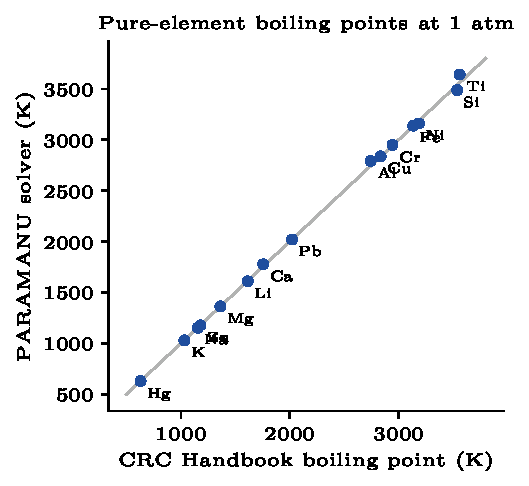
\includegraphics[width=\textwidth]{fig_validation.pdf}\end{minipage}
\end{center}
The largest boiling-point errors are for titanium (+81\,K, 2.3\%), silicon and aluminium ($\pm$49\,K), elements whose data are fitted over very wide temperature ranges; for the metals that carry the claims (iron, copper, lead, zinc, mercury) the error is at most 5\,K.

\subsection{The ladder}
The table of Chapter~\ref{ch:ladder} is the main result. Half-condensation temperatures at 1\,atm (K): W 3,000, Ti 2,825, Nd 2,350, Pt 2,325, Pd 2,300, Co 2,275, Fe 2,225, Al 2,200, Ca 2,100, Au 2,075, Mg 1,950, Si 1,925, Ni 1,850, Sn 1,725, Cu 1,700, Ga and Sb 1,675, Cr 1,650, S 1,500, Mn 1,375, Na 1,225, Ag 1,175, Cl and K 1,125, Bi and Pb 1,025, F 975, C 925, Li 850, Zn 675, In 650, Cd 475, P 400; mercury and nitrogen never reach 50\%.

\begin{figure}[H]
\centering
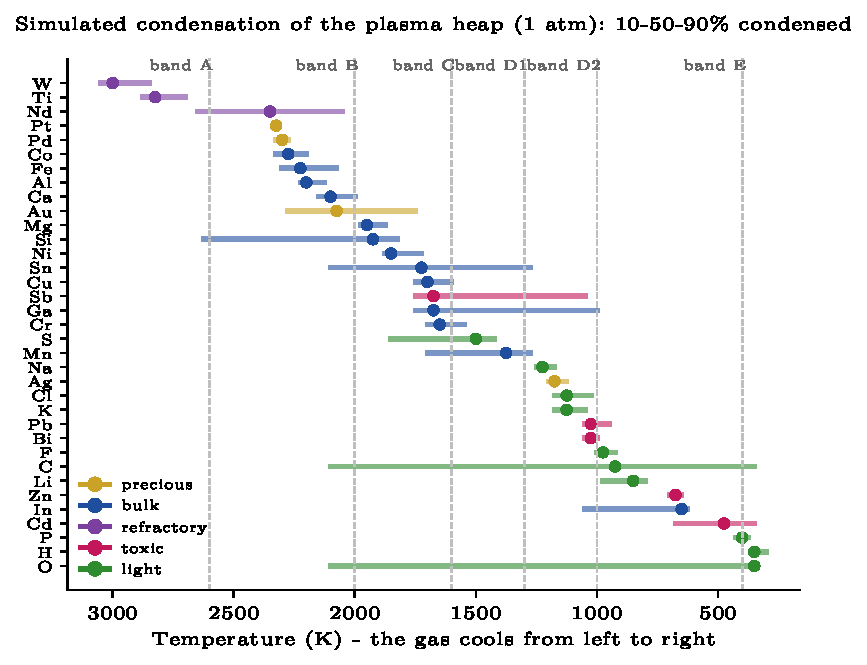
\includegraphics[width=\textwidth]{fig_ladder_simulated.pdf}
\caption{Simulated condensation at 1\,atm: temperatures at which 10\%, 50\% (dot) and 90\% of each element has condensed.}
\end{figure}

Key numbers: gold is 58.1\% in Band B and 41.9\% in Band C, 13.9\,ppm in the metal of its main band, 28 times the feed's 0.5\,ppm; palladium and platinum 100\% in Band B; zinc 100\% in Band E; lead 78.5\% in D2 and 21.5\% in E; cadmium 89\% in E; mercury 50\% still gaseous at 300\,K.

\paragraph{Every element in every band.} Share of each element collected in each band (\%), default feed, 1\,atm:
\input{tables/ladder_recovery}
\paragraph{How sharply each element condenses.} Temperatures at which 10\%, 50\% and 90\% of each element has condensed. A narrow range means a clean cut between bands; a wide range (silicon, carbon, oxygen) means the element is spread over several bands, usually because it forms several compounds.
\input{tables/ladder_T}
\paragraph{Mass per band.}
\input{tables/ladder_mass}
\begin{figure}[H]
\centering
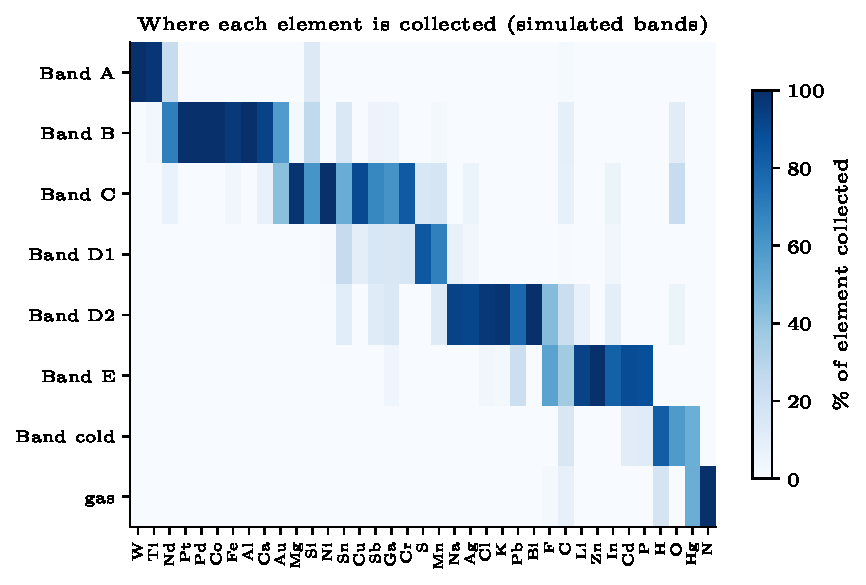
\includegraphics[width=\textwidth]{fig_ladder_recovery.pdf}
\caption{Share of each element collected in each simulated band.}
\end{figure}

\paragraph{The verdict on the original vision.}
\begin{center}
\small
\begin{tabular}{@{}>{\raggedright\arraybackslash}p{4.2cm}>{\raggedright\arraybackslash}p{8cm}>{\raggedright\arraybackslash}p{2.3cm}@{}}
\toprule
\textbf{Claim} & \textbf{What the simulation says} & \textbf{Verdict} \\
\midrule
The residue can be put fully in the gas phase & all gas at 2,890\,K (1\,atm), 2,630\,K (0.1\,atm), 3,190\,K (10\,atm) & supported \\
Elements separate into bands & clear bands, at lower temperatures than boiling points suggest & supported, revised \\
Precious metals are concentrated & Pd, Pt with iron; gold split iron/copper; 28-fold enriched & supported, revised \\
Toxic volatiles leave the precious band & in 5,000 feeds no Zn, Hg or Pb in a gold band (Pb after the D split); Cd at most 0.01\% & supported, revised \\
Mercury gathers at the cold end & 58\% still gaseous at 1\,atm; a trap is required & revised \\
Bands sit at fixed temperatures & every band moves with pressure & revised \\
The heap carries its own reductant & iron 100\% metallic with organics, 43\% without & supported \\
About 10.5\,MWh per tonne & 2.9\,MWh minimum to all gas; 10.5 is an upper bound & revised down \\
A sealed batch can be cooled slowly & impossible: wall radiation exceeds the batch energy in seconds & not supported \\
The heap is a plasma & 0.02\% ionized at 2,890\,K: a hot vapor & revised \\
\bottomrule
\end{tabular}
\end{center}

\subsection{The reductant, tested}\label{sec:reductant}
Repeating the ladder with the organics removed, halved, kept and doubled: without organics only 43\% of the iron condenses as metal; with half or more of the normal organics, all of it does. Nickel, copper, chromium, zinc and lead condense as metals in every case; silicon ends mostly as silica and silicon carbide.
The ratio $(C + H/2)/O$ and the share of each metal condensing as metal (not oxide, carbide or salt), as the organics are scaled:
\input{tables/reductant}
\begin{figure}[H]
\centering
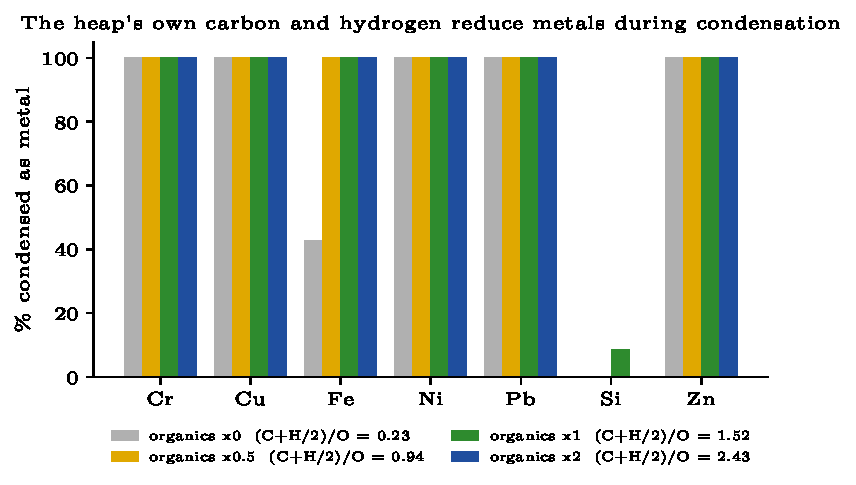
\includegraphics[width=0.85\textwidth]{fig_reductant.pdf}
\caption{Share of each metal condensing as metal as the organic fraction is varied.}
\end{figure}

\subsection{How complex waste comes apart}
Result~7 says where the heap ends up; this says how fast it gets there. Three stages:
\begin{enumerate}
\item \textbf{Organics crack at low temperature.} PVC releases its chlorine as HCl at 272--379\,\textdegree C; polyethylene and polypropylene decompose by about 480\,\textdegree C \citep{yuan2020}. What reaches the hot zone is small molecules and tar vapor.
\item \textbf{Mineral grains must be heated and vaporized: the slow step.} Heat reaches a small grain by conduction; a grain of diameter $d_0$ needs at least
\[
t = \frac{\rho d_0^2(\Delta h/12 + L/8)}{S_{\text{gas}} - S_{\text{surface}}},
\]
with $S = \int k\,dT$ the heat-conduction potential. For silica ($\Delta h = 3.44$\,MJ/kg to liquid at 2,900\,K, $L = 12.39$\,MJ/kg to vapor) in gas at 3,500\,K, a 10\,\textmu m grain needs 1.3\,ms; grains up to 27\,\textmu m vaporize in 10\,ms and 43\,\textmu m in 25\,ms. This is a lower bound: measured, 30\,\textmu m silicon grains evaporated to 90\% and 60\,\textmu m only to 30--40\% in a 50\,kW induction plasma \citep{gitzhofer1996}. Design rule: grind to about 20\,\textmu m or heat a molten film directly. The vaporization time of a silica grain (ms, lower bound) by size and gas temperature:
\input{tables/breakdown_particles}
\item \textbf{Molecules break in microseconds.} The hardest, CF\textsubscript{4} (from PFAS and fluoropolymers), lives 75\,\textmu s at 2,900\,K \citep{modica1968,cobos2023}, so a 25\,ms hot zone lasts over 300 lifetimes; its lifetime rises to 14\,ms at 2,200\,K, so every parcel must reach about 2,500\,K. European law asks incinerators for 850\,\textdegree C for two seconds (1,100\,\textdegree C for halogenated hazardous waste) \citep{eu2010ied}.
\end{enumerate}

\begin{figure}[H]
\centering
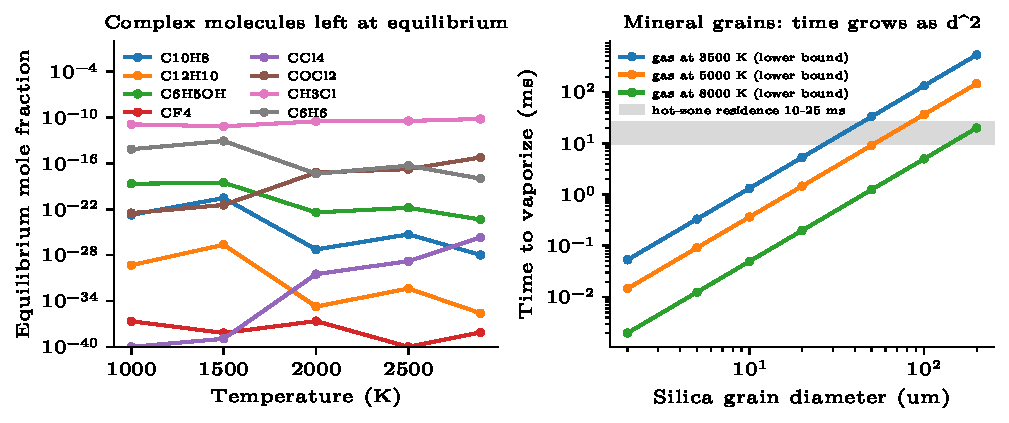
\includegraphics[width=\textwidth]{fig_breakdown.pdf}
\caption{Left: equilibrium mole fractions of complex molecules in the real heap. Right: time to vaporize a silica grain against the hot-zone residence time.}
\end{figure}

\subsection{Why the batch must be a pulse}\label{sec:chamber}
One tonne of residue as gas at 2,890\,K and 1\,atm fills 11,700\,m\textsuperscript{3}, a sphere 28\,m across, whose walls would radiate 1--3\,GW (emissivity 0.1--0.3) against a batch energy of only 4\,MWh. Even 10\,kg at 10\,atm radiates 15--46\,MW. This is the most important constraint the analysis added: the hot phase lasts tens of milliseconds, in a continuous or pulsed flow, as in flash Joule heating \citep{deng2021} and plasma spraying. The Saha equation gives ionization of about 0.02\% at 3,000\,K, 0.8\% at 5,000\,K and 11\% at 10,000\,K (upper bounds): at its all-gas temperature the heap is a hot vapor heated by plasma torches.
\input{tables/chamber_sizing}
\begin{center}
\begin{minipage}[t]{0.4\textwidth}\centering\textbf{Saha ionization at 1\,atm (upper bound)}\\[3pt]\input{tables/saha}\end{minipage}\hfill
\begin{minipage}[t]{0.52\textwidth}\centering\textbf{Heat each condenser removes}\\[3pt]\input{tables/condenser_duty}\end{minipage}
\end{center}

\subsection{Robustness: 5,000 random landfills}\label{sec:sweep}
\paragraph{Method.} Each of 5,000 feeds draws: every component mass (lognormal, 30\%), every trace concentration (lognormal, 60\%), the mercury content (about 2\,ppm, 60\%), the pre-treatment (0--30\%), the pressure (0.1, 1 or 5\,atm), every activity coefficient within its stated uncertainty, and one of the three chloride data sets. Each feed runs through the full ladder from 6,000 to 300\,K in 50\,K steps with full trace chemistry: 114 equilibrium states per feed, 570,000 in all. Each feed has a fixed random seed and can be reproduced individually.

\paragraph{Computing.} The final sweep ran on a rented cloud server (RunPod) with 10 cores, Python 3.10 and pinned library versions (Cantera 3.2.0, NumPy 2.2.6, SciPy 1.15.3, pandas 2.3.3), one worker per core: 0.41\,h of wall time, about 12,300 feeds per hour, about 3 core-seconds per feed, under one US dollar. A graphics processor would not help: each feed is a chain of dependent equilibrium solutions on CPU cores. Every finished feed is saved immediately so an interrupted sweep resumes; a feed over ten minutes is recorded as failed (none was).

\paragraph{Outcome.} All 5,000 feeds completed, and all 570,000 equilibrium states passed the certificate.
\begin{itemize}
\item \textbf{Zinc, mercury and lead reach no band that collects gold}, in none of the 5,000 feeds (all of which contain them). By the rule of three, the failure rate is below $3/5000 = 0.06\%$ at 95\% confidence, under the sampled input distributions. \emph{Caveat found in the review:} the sweep treats condensed metals as pure phases, so zinc and lead cannot dissolve in the iron and copper; with an ideal liquid alloy the gold band holds 0.009\% of the zinc and 0.5\% of the lead, and real copper alloys may hold more (a CALPHAD check is needed).
\item \textbf{Cadmium} reaches the gold bands only in traces: at most 0.01\%.
\item \textbf{Gold} is collected in the iron and copper bands: B and C together hold a median 100\% of it, and at least 99.3\% in 95\% of feeds at 1\,atm; Band B a median 60\%, Band C 34\%. Palladium and platinum stay with iron in Band B in 95\% and 94\% of feeds (the rest in Band A, at 5\,atm).
\item \textbf{Pressure sets the split}: gold's main band is B in 74\% of feeds at 1\,atm and 99\% at 5\,atm, but C (59\%) or D1 (40\%) at 0.1\,atm. The plant should run at 1\,atm or above.
\item \textbf{Chlorine data do not matter}: gold's median share in Band B is 61\%, 58\% and 61\% with the three chloride data sets.
\item \textbf{Mercury needs its trap}: median 58\% still gaseous at 300\,K at 1\,atm, 10\% at 5\,atm (41\% at the 95th percentile), all of it at 0.1\,atm.
\end{itemize}

\begin{center}
\small
\begin{tabular}{@{}>{\raggedright\arraybackslash}p{5.4cm}rrrr@{}}
\toprule
& \textbf{0.1\,atm} & \textbf{1\,atm} & \textbf{5\,atm} & \textbf{All} \\
\midrule
Feeds & 1,695 & 1,633 & 1,672 & 5,000 \\
Gold mainly in A / B / C / D1 (\% of feeds) & 0/1/59/40 & 0/74/26/0 & 1/99/0/0 & 0/58/28/14 \\
Gold in B+C, 5th percentile (\%) & 40 & 99 & 72 & 46 \\
T50 of Fe / Au (K, median) & 2000/1700 & 2250/2100 & 2450/2350 & -- \\
Feeds with lead in a gold band & 0 & 0 & 0 & 0 \\
Zinc or mercury in a gold band & none & none & none & none \\
Median mercury gaseous at 300\,K (\%) & 100 & 58 & 10 & 62 \\
\bottomrule
\end{tabular}
\end{center}

\paragraph{The sweep in numbers.} Claim by claim (a ``gold band'' collects at least 10\% of the gold):
\input{tables/sweep_claims}
Gold per band across all 5,000 feeds:
\input{tables/sweep_gold}
Spread of key quantities across the feeds:
\input{tables/sweep_quantiles}
Everything by pressure (shares are fractions of feeds; ``Au\_in\_\ldots'' are shares of the gold):
\input{tables/sweep_by_pressure}

\begin{figure}[H]
\centering
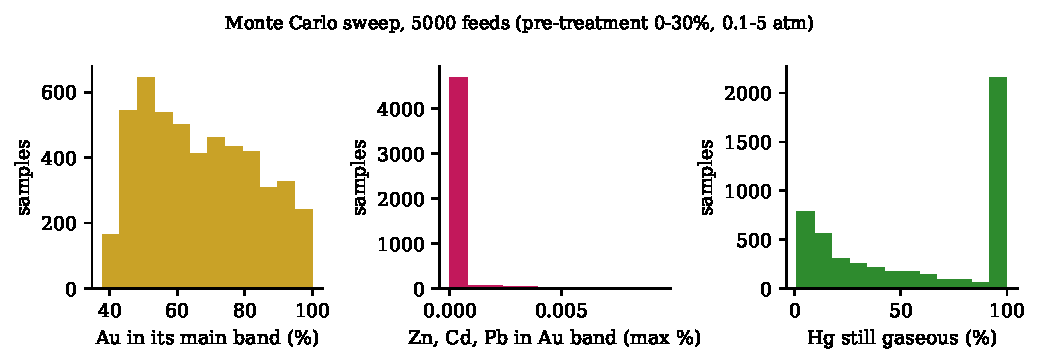
\includegraphics[width=\textwidth]{fig_sweep.pdf}
\caption{The 5,000-feed sweep.}
\end{figure}

\subsection{Numerical convergence and one-at-a-time sensitivity}
Halving the ladder step from 25 to 12.5\,K changes gold's share in Band B by one percentage point and the mercury left in the gas by $3\times10^{-6}$: the results are properties of the physics, not of the step. One-at-a-time changes show that the plastics content drives the energy ($\pm0.3$--$0.5$\,MWh/t for $\pm20\%$), pressure is the main lever for mercury (22\% left at 2\,atm, 100\% at 0.5\,atm), and halving or doubling all trace concentrations changes nothing, as Result~3 predicts for the dilute limit.
\input{tables/convergence}
\input{tables/sensitivity}
\begin{figure}[H]
\centering
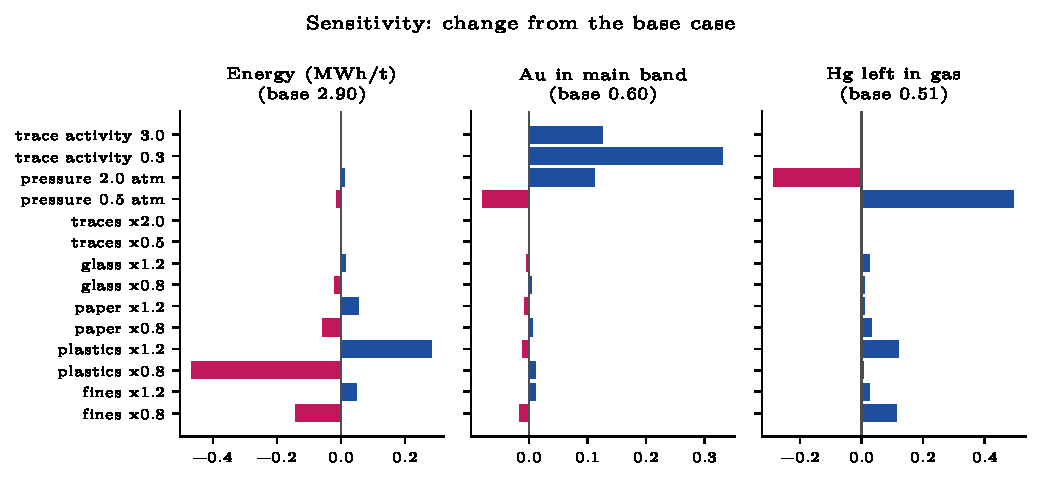
\includegraphics[width=\textwidth]{fig_sensitivity.pdf}
\caption{One-at-a-time sensitivity of energy, gold capture and mercury capture.}
\end{figure}

\subsection{Alloying}
Letting the liquid metals dissolve in one another (one ideal liquid-metal solution, a convex constraint like the gas) changes details, not conclusions: nickel condenses with iron at 2,525\,K instead of 1,850\,K, copper at 1,800 instead of 1,700\,K, and Band B becomes an iron--nickel--copper alloy holding 52\% of the gold and 57\% of the palladium. Zinc, cadmium, lead and mercury still stay out of the gold band, and the all-gas temperature is unchanged. The pure-phase and ideal-alloy models bracket real alloys.
\input{tables/alloy_T50}
\begin{figure}[H]
\centering
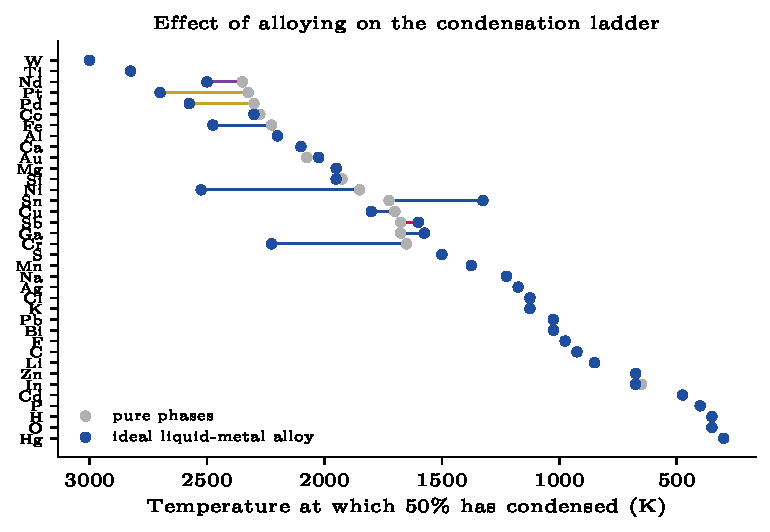
\includegraphics[width=0.85\textwidth]{fig_alloy.pdf}
\caption{Half-condensation temperatures with pure condensed phases and with an ideal liquid-metal alloy.}
\end{figure}

\subsection{Gold between iron and copper}\label{sec:gold}
Three findings, from full trace chemistry (script \texttt{15\_gold\_copper.py}):
\begin{enumerate}
\item \textbf{Chlorine does not move the precious metals.} In this hydrogen-rich gas chlorine stays as HCl; gold, silver, palladium and platinum land in the same bands with the least and the most volatile chloride data. Only cadmium moves, further from the gold.
\item \textbf{Palladium and platinum stay with iron} (Band B) in every case.
\item \textbf{Gold divides between the iron and copper bands.} Iron condenses first (2,000--2,600\,K), where gold's dislike of iron is weak (its activity coefficient in iron falls from 17 at 1,373\,K to about 1.4--2.3 at 2,000--2,250\,K); what iron does not capture dissolves in the copper condensing in Band C, which gold strongly prefers. With measured coefficients: 58\% in B and 42\% in C at 1\,atm; 36--82\% in B at the ends of the uncertainty; 84\% in B at 5\,atm; mostly C at 0.1\,atm. Both bands are alloys that copper and precious-metal smelters already refine, so the gold is recovered either way.
\end{enumerate}

Share of gold (\%) in each band under each scenario:
\input{tables/gold_scenarios}

\begin{figure}[H]
\centering
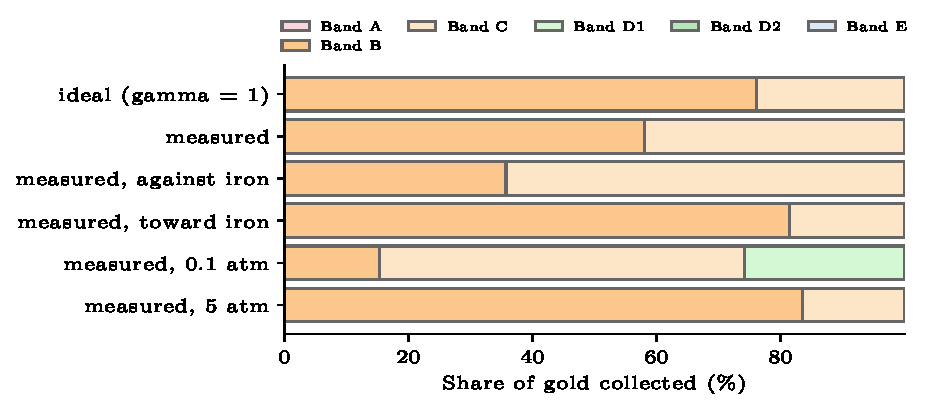
\includegraphics[width=0.9\textwidth]{fig_gold_copper.pdf}
\caption{Where gold is collected under different activity coefficients and pressures.}
\end{figure}

\subsection{The code against published measurements}\label{sec:benchmarks}
A model earns trust by predicting measurements it was not tuned on (script \texttt{14\_benchmarks.py}):
\begin{itemize}
\item \textbf{Vapor pressures} of lead and tin agree with the values used in vacuum refining \citep{jia2013} within 3\% (lead) and 9--18\% (tin), 800--1,300\,\textdegree C.
\item \textbf{The waste as its own reductant.} Electric-arc-furnace dust (mostly ZnO and magnetite, 5.6\% chlorine) reduced with coke at C/O = 0.16, 0.5, 0.8 and 1,300\,\textdegree C \citep{chang2022}: the model reproduces iron metallization (complete at 0.8, measured $>$90\%; none at 0.16, measured $\le$10\%). For zinc, equilibrium predicts full removal at every ratio while coke pellets removed 98.8\%, 88.5\% and about 50\%: solid coke reacts only where it touches the dust, and the same study's biomass pellets, whose reductant is a gas, removed 97.9\% even at 0.16. Equilibrium is the ceiling, and a gas-phase reductant, as in the heap, reaches it.
\item \textbf{Gold between iron and copper} \citep{yamaguchi2006}: the activity coefficients predict a distribution ratio of 0.0033 against 0.0071--0.013 measured at 1,373\,K: the right direction, overstated by a factor of 2--4, so the model's gold split errs, if at all, against the iron band.
\end{itemize}

\paragraph{The benchmark data.} Vapor pressures (model against literature, ratio 1 = exact):
\input{tables/bench_vp}
Electric-arc-furnace dust at 1,300\,\textdegree C, with the nitrogen sweep of the experiment and in a closed system:
\input{tables/bench_eaf}
Gold and silver between liquid iron and copper at 1,373\,K ($L$ = distribution ratio Fe/Cu):
\input{tables/bench_gold}
Silver's predicted ratio is 6.5 times the measured one, the opposite direction to gold; its coefficients are therefore the less reliable, which matters little because silver collects in Band D2 regardless (96\% of feeds).

\begin{figure}[H]
\centering
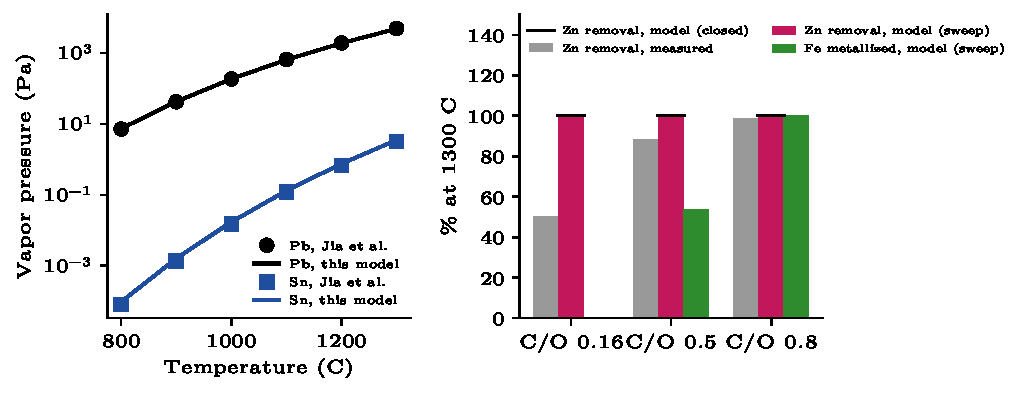
\includegraphics[width=\textwidth]{fig_benchmarks.pdf}
\caption{Benchmarks: vapor pressures (left); electric-arc-furnace dust reduction, measured bars grey (right).}
\end{figure}

\subsection{Limits of the model}
\begin{itemize}
\item \textbf{Trace data are the weakest part.} No open data exist for gold chlorides (AuCl computed, $\pm$13\,kJ/mol); gold's activity coefficient in liquid iron is extrapolated from alloys with at least 44\% gold and from up to 1,573\,K; in copper it rests on one tabulated value; platinum in iron and copper and palladium in copper are unmeasured (treated as ideal); dissolved carbon's effect on gold is unknown; traces dissolve only in condensing metals, not in slag. Each is bracketed in the sweep.
\item Alloys are ideal solutions and oxides pure phases (CALPHAD models would refine band compositions).
\item \textbf{Equilibrium at every step}: no nucleation, kinetics or aerosols; grey-gas radiation.
\end{itemize}

%=====================================================================
\section{The Journey of Each Element}\label{ch:journeys}
%=====================================================================
This chapter follows the elements that matter most from the hot zone to their collectors, with the numbers of the default feed at 1\,atm and of the 5,000-feed sweep.

\paragraph{Gold.} Enters at about 0.5\,ppm (an assumption; no measurement in landfill fines exists). In the hot zone it is atomic gas, with some AuCl. It condenses by dissolving: first in the liquid iron condensing at 2,000--2,600\,K (Band B), where its dislike of iron is weak at those temperatures, then in the copper condensing at 1,600--2,000\,K (Band C), which it strongly prefers. Default feed: 58.1\% in B, 41.9\% in C, half-condensed at 2,075\,K, 13.9\,ppm in the metal of Band B (28 times the feed). Sweep: median 60\% in B and 34\% in C; B+C at least 99.3\% in 95\% of feeds at 1\,atm. In organic-rich feeds some gold passes C into D1 (1,300--1,600\,K), never into lead's D2. What decides the split: gold's activity coefficient in liquid iron (86\% of the variance at 1\,atm). Refining: both bands are collector alloys that precious-metal refineries process; condensation cannot split gold from iron (26 stages).

\paragraph{Palladium and platinum.} 100\% in Band B with iron in the default feed; in the sweep, B in 95\% (Pd) and 94\% (Pt) of feeds, Band A in the rest (at 5\,atm, where everything condenses hotter). With an ideal alloy they condense at 2,575 and 2,700\,K. Refining with the iron-band metal.

\paragraph{Silver.} Condenses late (half at 1,175\,K) in Band D2 with the salts: 91.2\% in D2, 5.3\% in C, 3.5\% in D1; in the sweep, D2 in 96\% of feeds. Silver is separated from gold by physics: $\alpha \approx 73$ at 2,000\,K, about two stages.

\paragraph{Iron.} The bulk metal: 96.1\% in Band B, as metal thanks to the waste's own reductant (43\% metallic without organics), half-condensed at 2,225\,K. The collector for gold, palladium and platinum.

\paragraph{Copper.} 90.1\% in C, 9.9\% in D1, half at 1,700\,K (1,800\,K with alloying). The second gold collector. Separable from nickel in about 3.5 stages.

\paragraph{Lead.} The case the adversary tested hardest. Half-condensed at 1,025\,K: 78.5\% in D2, 21.5\% in E, never in a gold band once Band D is split. In the first design (one Band D at 1,000--1,600\,K), organic-rich feeds brought gold down into lead's band; lead itself never moved (Chapter~\ref{ch:verification}).

\paragraph{Zinc.} 100\% in Band E, half at 675\,K, 1,400\,K below gold. Never in a gold band in 5,000 random and 1,664 adversarial feeds (the closest the adversary got was a 700\,K gap). Separates from iron in a single stage.

\paragraph{Cadmium.} 88.9\% in E and 11.1\% at the cold end, half at 475\,K. Traces reach the gold bands dissolved in the metals: at most 0.01\% in 5,000 feeds and 0.025\% in the adversarial search. Stored as cadmium sulfide.

\paragraph{Mercury.} At about 2\,ppm, too dilute to condense: half is still gas at 300\,K at 1\,atm (median 58\% in the sweep), 10\% at 5\,atm, all at 0.1\,atm. Caught by a sulfur-impregnated carbon trap as mercury sulfide, the form of its ore; European law already requires that form \citep{eu2017mercury}. Its amount in the gas is set by the mercury content and the plastics, not by any uncertain data.

\paragraph{Tin and antimony.} Spread over several bands (tin: 14\% B, 51\% C, 24\% D1, 11\% D2), because they dissolve in several host metals; tin from copper would need 258 stages. They follow the copper and iron streams to refining.

\paragraph{Chlorine, sodium, potassium.} Condense together as salts in D2 (chlorine 96.6\%, sodium 92.3\%, potassium 97.7\%). In the hot, hydrogen-rich gas chlorine stays as HCl, which is why it does not carry the precious metals away.

\paragraph{Silicon, aluminium, calcium, magnesium.} The mineral bulk: silicon over A, B and C (as silica, silicon carbide and in alloys), aluminium 99.8\% and calcium 92.5\% in B as oxides, magnesium 98.4\% in C. Most of it becomes glass unless a market exists.

\paragraph{Carbon, hydrogen, oxygen, nitrogen.} The reductant and the fuel: water at the cold end, methane (or H\textsubscript{2} and CO if quenched) and nitrogen to cylinders, carbon partly as carbides in the metal bands.

%=====================================================================
\section{Rechecking the Computation: Testing the Model Itself}\label{ch:verification}
%=====================================================================
The sweep shows that the claims survive realistic variation \emph{if the model is right}. It cannot show the model is right, because all its states came from one solver and one database. This chapter tests the model itself. The rule for every test: \textbf{it must not share the weakness it checks}.

\subsection{A certificate for every equilibrium state}\label{sec:certificate}
Result~2 does more than guarantee the equilibrium exists; its dual form tells how to \emph{recognize} it without trusting whoever computed it \citep{boyd2004}. A state with gas amounts $n_k$ and condensed amounts $n_c$ is the equilibrium if and only if one vector of element potentials $\lambda$ satisfies:
\begin{align*}
\ln x_k &= a_k\cdot\lambda - g_k - \ln(P/P_0) && \text{for every gas species (all have the potential of their atoms)},\\
a_c\cdot\lambda &= g_c && \text{for every condensed phase present},\\
a_c\cdot\lambda &\le g_c && \text{for every condensed phase absent (nothing supersaturated)},\\
\textstyle\sum_k a_{ik}n_k + \sum_c a_{ic}n_c &= b_i && \text{for every element (no atom lost or made)}.
\end{align*}
The certificate (\texttt{equilibrium.certify}) fits $\lambda$ to the amounts by least squares, so it uses nothing from the solver but the answer, and accepts the state only if every condition holds to $10^{-4}$. If the batch has no gas at all, the gas condition becomes ``the gas phase would be unstable'', i.e.\ the predicted mole fractions sum to at most one. Because the equilibrium is unique, a state that passes \emph{is} the equilibrium; a state that fails is wrong, however confident its solver. \textbf{Result:} all 570,000 major-element states of the sweep and every step of the default ladder pass; the Cantera backup was needed for none. \emph{Scope:} the certificate covers the major-element equilibrium; the trace metals, gold among them, are placed afterwards by the dilute-limit solver, which the automated tests check against the full solver; remnants below $10^{-9}$ of the gas are assigned to the current collector. A student exercise: delete one condensed phase from a state and watch the certificate fail on the element balance (\texttt{docs/STUDENT\_GUIDE.md}, chapter 11).

\subsection{What the checks found and fixed}\label{sec:defects}
Three defects in the computation and one in the design were found, each by a check of this chapter, never by the sweep, whose statistics looked normal each time.
\begin{enumerate}
\item \textbf{Unconverged steps.} Comparing every ladder state with Cantera showed that PARAMANU's solver did not converge at 43 of 229 ladder steps below 1,850\,K. The cause was numerical: after most of the batch had condensed, remnants at parts per billion (for example $10^{-4}$\,mol of titanium in 38,000\,mol of gas) were solved together with the majors, and the balance could not be closed to the required relative accuracy for both. \emph{Fix:} elements below 1\,ppm of the gas are placed by the dilute-limit solver at the majors' certified potentials (Result~3). Nothing is dropped; every atom is still placed and counted.
\item \textbf{A second solver that is confidently wrong.} Cantera's solver, added as a backup, reported convergence at 0.1\,atm, with a balance closed to $10^{-15}$, for states that are not the equilibrium: graphite beside 66\% steam with no carbon monoxide; zinc sulfate, sodium superoxide and liquid iron carbonyl at 1,650\,K. Used blindly, they put zinc, lead and mercury entirely into Bands C and D in 183 of 5,000 feeds. The certificate rejects them by huge margins (for one feed at 1,450\,K Cantera's gas violates the first condition by 168 in $\ln x$, against a tolerance of $10^{-4}$). \emph{Lesson:} two solvers agreeing is evidence, a solver saying ``converged'' is not, and the certificate decides. \emph{Fix:} every state must pass the certificate; the affected sweep was discarded and rerun.
\item \textbf{A missing phase.} The certificate then found rare states where PARAMANU's own solver had left out graphite (supersaturated by a factor of 1.4) in carbon-rich feeds at 1,400--1,450\,K and 0.1\,atm. \emph{Fix:} the NASA CEA phase-set iteration (\texttt{gibbs.refine}) adds the missing phase and solves again. Before: 569,696 of 570,000 states certified; after: all. The claims were the same before and after.
\item \textbf{A design flaw for lead}, found by the adversarial search (Section~\ref{sec:adversary}), fixed by splitting Band D.
\end{enumerate}

\subsection{A second solver}
Cantera's multiphase solver \citep{cantera2023} implements the VCS algorithm of \citet{smithmissen1982}, written independently of PARAMANU's. Both were given the same element totals for the whole batch from 3,000 to 400\,K and at every ladder state. Cantera converged at 51 of 53 states and at every one found the same condensed phases as PARAMANU; amounts agree within 0.19\% (condensed) and $2.4\times10^{-5}$ (major gas species). PARAMANU's own solver, with no backup, converged and passed the certificate at all 53 states.
Every state compared (``whole heap'': the full batch, closed, at each temperature; ``ladder step'': the gas left at each step of a 100\,K ladder, major elements):
\input{tables/verif_solver}

\subsection{A second database}\label{sec:seconddb}
The data could be wrong in a way no solver check would reveal. The major-element ladder was recomputed with the full NASA CEA database \citep{mcbride2002}: 558 gas and 366 condensed species with their own NASA-9 fits, instead of the 428 gas and 250 condensed NASA-7 species used elsewhere (nine records with inconsistent temperature ranges were skipped). Of 23 elements, 21 land in the same main band, and the median change in half-condensation temperature is 0\,K. The exceptions: lithium moves from E to D2 (+200\,K); fluorine stays in the gas with the NASA-9 data; phosphorus condenses 350\,K higher but in the same band. Iron, copper, nickel, zinc, lead and mercury are identical. (The precious metals are outside both NASA sets; their data are tested by the benchmarks.)
\input{tables/verif_data}

\subsection{An adversary that tries to break the claims}\label{sec:adversary}
A random sweep samples typical feeds; a failure that needs an unusual combination can hide between its samples. So an optimizer was set to break the claims (script \texttt{20\_falsification.py}).
\paragraph{How.} For each claim, differential evolution \citep{storn1997} searched all 56 uncertain inputs at once, over ranges wider than the sweep's: each component mass from a third to three times its default, each trace and the mercury content from a sixth to six times, pre-treatment 0--30\%, pressure continuously, every activity coefficient across its uncertainty, all three chloride data sets. It was rewarded for moving a toxic metal into a band that collects at least 10\% of the gold, and, where that share was exactly zero, for narrowing the gap between gold's and the metal's condensation temperatures (a continuous ``distance to failure''). A claim is falsified if any input puts more than 1\% of zinc, mercury or lead (0.1\% of cadmium) into a gold band. Each claim got 1,664 attempts (26 generations of 64), 6,656 in all, 74 minutes on a cloud server.

\paragraph{First design: lead failed.} Zinc and mercury never reached a gold band and cadmium stayed below 0.025\%, but for lead 162 of 1,664 attempts exceeded 1\%, the worst with 49\% of the lead in a gold band. The random sweep had missed it because it needs an unusual combination: two to three times the usual paper and plastics, whose CO and H\textsubscript{2} dilute the metal vapor, so gold condenses later (lower $yP$, Result~3) and 10--40\% of it passes the copper band into Band D, then 1,000--1,600\,K, where lead collects.

\paragraph{The diagnosis.} Recomputing 17 such feeds (ten from the search, and the seven lead cases the sweep had found) showed the cause: the stray gold condenses \emph{entirely} between 1,300 and 1,600\,K, where \emph{no} lead condenses, and the lead entirely below 1,300\,K, where no gold remains. Lead never moved toward gold; the band was too wide.

\noindent The 17 feeds recomputed in the diagnosis (first design; share of each element that condenses in the upper and lower halves of the old Band D):
\begin{center}
\footnotesize
\begin{tabular}{@{}llrrrrrr@{}}
\toprule
\textbf{source} & & \textbf{P (atm)} & \textbf{pre-treat} & \textbf{Au 1,300--1,600\,K} & \textbf{Pb 1,300--1,600\,K} & \textbf{Au 1,000--1,300\,K} & \textbf{Pb 1,000--1,300\,K} \\
\midrule
adversary & 1 & 1.17 & 0.06 & 11.1\% & 0.0\% & 0.0\% & 49.1\% \\
adversary & 2 & 1.01 & 0.06 & 25.0\% & 0.0\% & 0.0\% & 20.0\% \\
adversary & 3 & 1.31 & 0.05 & 11.5\% & 0.0\% & 0.0\% & 40.9\% \\
adversary & 4 & 1.24 & 0.07 & 25.9\% & 0.0\% & 0.0\% & 34.8\% \\
adversary & 5 & 1.12 & 0.05 & 21.5\% & 0.0\% & 0.0\% & 45.7\% \\
adversary & 6 & 1.05 & 0.08 & 24.7\% & 0.0\% & 0.0\% & 33.9\% \\
adversary & 7 & 1.21 & 0.06 & 23.1\% & 0.0\% & 0.0\% & 44.2\% \\
adversary & 8 & 1.17 & 0.05 & 22.3\% & 0.0\% & 0.0\% & 38.2\% \\
adversary & 9 & 1.35 & 0.09 & 11.6\% & 0.0\% & 0.0\% & 45.0\% \\
adversary & 10 & 1.42 & 0.08 & 20.6\% & 0.0\% & 0.0\% & 39.1\% \\
sweep & 1124 & 1.0 & 0.28 & 16.1\% & 0.0\% & 0.0\% & 32.8\% \\
sweep & 1885 & 0.1 & 0.14 & 27.2\% & 0.0\% & 0.0\% & 0.8\% \\
sweep & 2103 & 1.0 & 0.28 & 13.6\% & 0.0\% & 0.0\% & 33.3\% \\
sweep & 2722 & 0.1 & 0.18 & 37.6\% & 0.0\% & 0.0\% & 10.7\% \\
sweep & 3763 & 1.0 & 0.26 & 15.1\% & 0.0\% & 0.0\% & 42.4\% \\
sweep & 4479 & 1.0 & 0.20 & 15.5\% & 0.0\% & 0.0\% & 42.0\% \\
sweep & 4670 & 0.1 & 0.16 & 16.5\% & 0.0\% & 0.0\% & 16.6\% \\
\bottomrule
\end{tabular}
\end{center}
In every row the gold column below 1,300\,K and the lead column above it are zero. In all 17 feeds the lead's half-condensation temperature was 950\,K.

\paragraph{Remedies tested on the worst feed} (49\% of its lead in a gold band):
\begin{center}
\small
\begin{tabular}{@{}>{\raggedright\arraybackslash}p{5cm}>{\raggedright\arraybackslash}p{6.2cm}>{\raggedright\arraybackslash}p{3.2cm}@{}}
\toprule
\textbf{Remedy} & \textbf{How it works} & \textbf{Gold in lead's range} \\
\midrule
Split Band D at 1,300\,K (D1, D2) & one more condenser stage; D1 catches the gold tail, D2 the lead & 0\% (all 17 feeds) \\
Raise pressure to 5\,atm & higher $yP$ pulls gold back to B and C (Result~3) & 0\% \\
Keep organics normal (blend feed or pre-pyrolyse) & removes the dilution & 0\% \\
Add copper-rich scrap (4$\times$) & more copper collects gold in C & 11\% $\to$ 4\%: not enough alone \\
Refinery safety net & lead bullion is the classic gold collector (fire assay, Parkes, cupellation) & gold not lost, only rerouted \\
\bottomrule
\end{tabular}
\end{center}

\paragraph{Revised design: no failure.} Band D was split, and the \emph{whole} search was run again on the revised design: 0\% of zinc, mercury and lead in any gold band in 1,664 attempts each, and at most 0.025\% of the cadmium (limit 0.1\%); 6,656 feeds, none failing to compute. The 5,000-feed sweep, rerun on the revised design, also shows no lead in any gold band. The split is the remedy that needs no knowledge of the feed; pressure and feed blending are backups.

\noindent The search on the revised design, claim by claim (a ``gold band'' collects at least 10\% of the gold; the T50 gap is gold's half-condensation temperature minus the metal's):
\input{tables/falsification}
Zinc and mercury never came within 700 and 1,350\,K of gold; lead within 650\,K, now in its own band; cadmium's small traces are dissolved in the metals, not condensed with them.

\subsection{Which uncertainties matter (Sobol indices)}
The first-order Sobol index of an input is the share of an output's variance it explains alone \citep{sobol2001,saltelli2008}. The indices were estimated from the sweep's own feeds with the given-data method \citep{plischke2013}: sort feeds by the input, cut into 25 equal bins, take the variance of the bin means; the estimator's bias is measured on randomly shuffled inputs and subtracted (script \texttt{21\_global\_sensitivity.py}). Every feed's inputs are regenerated from its seed.
\begin{itemize}
\item \textbf{Across all feeds, pressure dominates} every gold and mercury result (58--84\% of the variance). Pressure is an operating choice, not an uncertainty.
\item \textbf{At a fixed 1\,atm, one uncertain number dominates the gold results}: gold's activity coefficient in liquid iron explains 86\% of the variance of gold's share in Band B and 77\% of its half-condensation temperature.
\item Mercury left in the gas is set by the mercury content (65\%) and plastics (17\%); cadmium traces in the gold bands by pre-treatment (69\%).
\item The chloride data, the other 28 activity coefficients and the trace concentrations each explain less than 2\% (the largest is 1.3\%).
\end{itemize}
\textbf{Consequence:} one measurement, gold's activity coefficient in liquid iron near 2,000\,K, would remove most of the remaining uncertainty in where gold is collected. It is pre-registered as P11.

\noindent All significant first-order indices, the four largest per output (``all'': all 5,000 feeds; ``1 atm'': the 1,633 feeds at 1\,atm):
\input{tables/sobol}
The sum of all first-order indices close to one (as for gold's share in Band B at 1\,atm) means the inputs act almost independently; a sum well below one (gold in B+C at 1\,atm, 0.28) means that output hardly varies and what little variation there is comes from combinations of inputs.

\subsection{Reproducibility on another machine}
Twenty sweep feeds, drawn at random with a fixed seed, were recomputed on a different computer (a 2-core workstation) and compared with the published table from the cloud server: across 108 metrics per feed the largest difference was $1.1\times10^{-13}$ (floating-point rounding), and every main band was identical (script \texttt{19\_reproducibility.py}).

\subsection{Predictions registered before experiment}
A result counts most when its passing mark was fixed before the measurement \citep{nosek2018}. Thirteen predictions for the first experiments are fixed in \texttt{docs/PREREGISTRATION.md} (its git history is the record they were not changed):
\begin{center}
\small
\begin{tabular}{@{}l>{\raggedright\arraybackslash}p{6.2cm}>{\raggedright\arraybackslash}p{3.1cm}>{\raggedright\arraybackslash}p{4.2cm}@{}}
\toprule
& \textbf{Prediction} & \textbf{Passes if} & \textbf{Counts against if} \\
\midrule
P1 & every element balance closes & within 3 std.\ uncertainties & it does not (fix first) \\
P2 & energy to all gas $\ge$2.90\,MWh/t & measured $\ge$2.6 & below 2.6\,MWh/t \\
P3 & iron in Band B is metal & $\ge$90\% metallic & $<$50\% \\
P4 & T50 order Fe 2,225 $>$ Au 2,075 $>$ Cu 1,700 $>$ Pb 1,025 $>$ Zn 675 $>$ Cd 475\,K & order kept, $\pm$150\,K & Zn, Cd or Hg above Au or Cu; off by $>$150\,K \\
P5 & no Zn, Hg or Pb in a gold band & $<$1\% each & $\ge$1\% of any \\
P6 & cadmium in gold bands $\le$0.01\% & $<$0.1\% & $\ge$0.1\% \\
P7 & gold in B+C 100\% & $\ge$95\% & $<$90\% \\
P8 & gold in B 58\% (feeds 40--83\%) & 20--95\% & outside \\
P9 & Pd, Pt in B $\sim$100\% & $\ge$90\% & $<$70\% \\
P10 & 1$\to$5\,atm raises gold's T50 and share in B & both rise & either falls \\
P11 & $\gamma$ of gold in liquid iron 1.4--2.3 (1,900--2,250\,K) & 0.5--7 & outside: P8 recomputed \\
P12 & CF\textsubscript{4} destroyed at $\ge$2,600\,K, 25\,ms & $<$0.01\% leaves & $\ge$0.01\% \\
P13 & the adversary's organic-rich feed: gold in D1, lead in D2 & $<$1\% overlap & $\ge$1\% \\
\bottomrule
\end{tabular}
\end{center}

\subsection{Summary of all tests}
\begin{center}
\small
\begin{tabular}{@{}>{\raggedright\arraybackslash}p{3.4cm}>{\raggedright\arraybackslash}p{4.2cm}>{\raggedright\arraybackslash}p{6.8cm}@{}}
\toprule
\textbf{Test} & \textbf{Would catch} & \textbf{Result} \\
\midrule
Certificate & any state not the equilibrium & all 570,000 + 228 states pass \\
Second solver & errors in the solver & same phases at all 51 converged states; within 0.19\% \\
Second database & errors in the data & 21 of 23 elements same band; median $\Delta T_{50}$ 0\,K \\
Published measurements & wrong data or chemistry & Pb/Sn within 3\% / 9--18\%; iron pattern; gold partition within 2--4$\times$ \\
Adversarial search & failures the sweep misses & broke the first design (lead); none after the D split \\
Sobol indices & hidden dependence & one coefficient sets gold's split; pre-registered \\
Second machine & hardware/software dependence & $1.1\times10^{-13}$; identical bands \\
Pre-registration & fitting after the fact & 13 predictions fixed in advance \\
\bottomrule
\end{tabular}
\end{center}

%=====================================================================
\section{Catalysts: What They Can and Cannot Do}\label{ch:catalysts}
%=====================================================================
\textbf{In the hot zone, no catalyst helps}, for three independent reasons (script \texttt{17\_catalysts.py}):
\begin{enumerate}
\item \textbf{It cannot change the outcome} (Result~8).
\item \textbf{It is not needed.} The slowest molecule, CF\textsubscript{4}, lives 80\,\textmu s at 2,890\,K, so the 25\,ms hot zone gives a Damk\"ohler number of 314 (53 at 2,600\,K; about 2 only at 2,200\,K, where the remedy is more heat, not a catalyst).
\item \textbf{It would not survive.} A metal surface evaporates at the Hertz--Knudsen rate $J = \alpha p^{\text{sat}}\sqrt{M/2\pi RT}$; at 2,890\,K a 5\,nm catalyst particle lasts 2.4\,\textmu s (nickel), 1.8\,\textmu s (iron), 2.8\,\textmu s (palladium) or 0.5\,ms (platinum); a 1\,mm nickel pellet half a second. The plasma-catalysis field itself places catalysts downstream of warm plasmas \citep{bogaerts2020}.
\end{enumerate}
\noindent Lifetime of catalyst metals at 2,890\,K (Hertz--Knudsen evaporation):
\input{tables/cat_survival}
\textbf{What does speed up the process} is not chemistry but heat into grains: \emph{grind finer} (time $\propto d^2$: 40$\to$20\,\textmu m is four times faster); \emph{more hydrogen} (the best heat conductor among plasma gases \citep{mauer2025}); and \emph{the waste's own carbon, a reagent}: SiO\textsubscript{2} + C $\to$ SiO + CO brings the SiO vapor pressure to 0.1\,atm at 1,811\,K instead of 2,874\,K, about 1,100\,K lower. In full:
\input{tables/cat_carbo}

\textbf{At the cold end, catalysts are essential}, in this order along the gas path: tar reforming (Ni, dolomite, olivine, 700--900\,\textdegree C, $>$95\% with dolomite or olivine \citep{jayanarasimhan2024}); dioxin destruction (V\textsubscript{2}O\textsubscript{5}--WO\textsubscript{3}/TiO\textsubscript{2}, 180--250\,\textdegree C, 98--99.9\% \citep{neuwahl2019}); water--gas shift (Fe--Cr, Cu--ZnO; chlorine must be removed first \citep{argyle2015}); methanation (Ni; sulfur below 0.1\,ppm). Three rules: \emph{clean before catalysing} (dust, tar, HCl, NH\textsubscript{3}, HCN, alkali, metals, sulfur, then shift); \emph{quench through the dioxin window} (450 to below 200\,\textdegree C within about a second \citep{epa2006dioxin}); \emph{do not rely on a catalyst for mercury} in this reducing gas: use the sulfur trap.

%=====================================================================
\section{The Value--Harm Slider}\label{ch:slider}
%=====================================================================
Atomizing everything does not mean purifying everything. An element $i$ with market value $V_i$, monetized harm $H_i$ and recovery cost $C_i$ is purified if and only if $V_i + sH_i > C_i$, where the operator's slider $s\in[0,1]$ runs from Commercial (0) to Nature (1); otherwise it is vitrified as future ore. The cost follows the Sherwood relation $C_i = K(c_i^{\text{eff}})^{-b}$ \citep{sherwood1959,johnson2007} in the band condensate, far richer than the heap. Each element switches on at $s^\ast_i = \max(0,(C_i-V_i)/H_i)$, so the purified set only grows as $s$ rises. With the baseline's illustrative inputs, mercury, cadmium and chromium switch on almost at once, arsenic at 0.105 and fluorine at 0.716.

\paragraph{Why the threshold only moves one way.} Rearranging $V_i + sH_i > C_i$ gives $s > (C_i - V_i)/H_i$. Because harm $H_i$ is never negative, $V_i + sH_i$ never falls as $s$ rises, so an element purified at some $s$ stays purified at any larger $s$: moving the slider toward Nature can only add elements to the purified set and can only increase the harm avoided. In the Atomize-First design the slider acts on band condensates and traps, which are far richer than the heap, so the Sherwood cost $C_i$ is lower than for the same element in raw waste; with the baseline inputs, mercury and arsenic are stabilized at every slider position above about 0.11.
\begin{figure}[H]
\centering
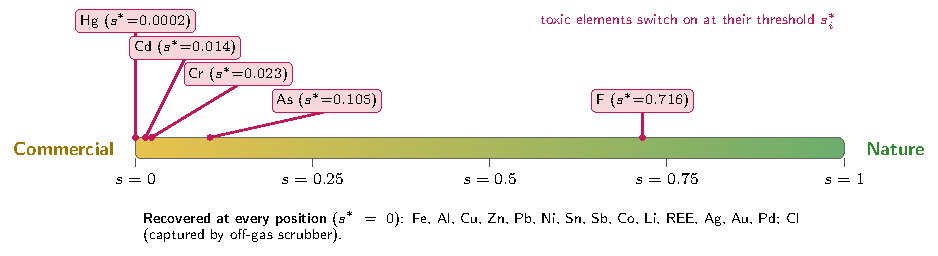
\includegraphics{fig_slider.pdf}
\caption{Activation thresholds on the Commercial--Nature slider (illustrative inputs from the baseline model).}
\end{figure}

%=====================================================================
\section{Energy}\label{ch:energy}
%=====================================================================
\paragraph{Upper bound.} Taking one wet tonne to single atoms at 5,000\,K costs about 10.5\,MWh (12.6 with 10\% ionized), from enthalpies of formation.
\begin{center}
\small
\begin{tabular}{@{}lrrr@{}}
\toprule
\textbf{Step} & \textbf{Mass (kg)} & \textbf{MJ/kg} & \textbf{MWh} \\
\midrule
Drying (evaporate moisture) & 250 & 2.8 & 0.20 \\
Atomize soil and glass (SiO\textsubscript{2} proxy) & 465 & 30.9 & 4.00 \\
Atomize plastics (polyethylene proxy) & 135 & 84.2 & 3.16 \\
Atomize paper and wood (cellulose proxy) & 90 & 53.6 & 1.34 \\
Atomize other residue & 21 & 15.0 & 0.09 \\
Heat 64,400\,mol of atoms to 5,000\,K & -- & -- & 1.75 \\
\midrule
\textbf{Total (atomize and heat)} & & & \textbf{10.5} \\
Optional: ionize 10\% of atoms (about 12\,eV each) & & & +2.1 \\
\bottomrule
\end{tabular}
\end{center}
\paragraph{What is actually needed.} Separation needs a gas, not atoms. The equilibrium calculation puts the whole residue in the gas phase at 2,890\,K and 1\,atm for \textbf{2.9\,MWh per tonne}, mostly as CO, H\textsubscript{2} and SiO: about \textbf{120\,MW} for 1,000 tonnes per day before wall losses. Pre-treatment is a moderate dial (3.0\,MWh/t with none, 2.5 with 30\% removed). The full calculation by pressure and pre-treatment:
\input{tables/energy_envelope}
How the energy builds up as the tonne is heated at 1\,atm (relative to the feed at 298\,K; negative at 300\,K because the equilibrium products there are more stable than the feed):
\input{tables/energy_curve}
\begin{figure}[H]
\centering
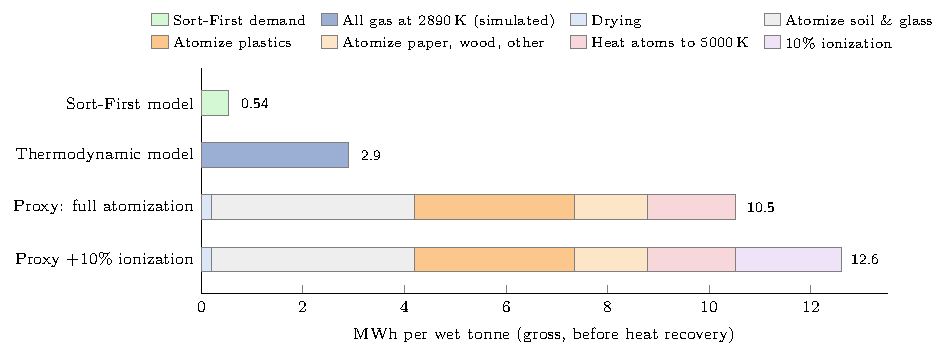
\includegraphics[width=\textwidth]{fig_energyenv.pdf}
\caption{Gross energy per wet tonne: Sort-First baseline, the simulated all-gas state, and the full-atomization upper bound.}
\end{figure}
Three observations shape efficiency work. Pre-treatment is a real but moderate dial: sending everything (0\% pre-treatment) needs 3.0\,MWh per tonne, and removing 30\% of the mass lowers it to 2.5\,MWh. The gross energy is small next to wall losses, so how long the gas stays hot matters more than how much is vaporized. And most of the energy is not destroyed: it comes back as high-temperature heat when the gas condenses (42\% of the condenser heat is released above 2,000\,K) and as chemical energy in the fuel gas, so heat recovery is the first efficiency target.
\paragraph{Delivering it is the hardest engineering problem.} 2.9\,MWh/t (4.1\,kWh or 15\,MJ per kg of dry residue) is the gross enthalpy of the all-gas state without heat recovery. Powder blown through a torch jet has given ``generally disappointing'' efficiencies; heating the material directly does better: a centrifugal plasma furnace vaporized silica with carbon at 9.3\,kWh/kg \citep{sayce1976}, about 2.3 times the minimum, so a 1,000\,t/day plant needs about 280\,MW. Design consequences: heat a molten film or bath directly; if powder is injected, grind it to 10--40\,\textmu m.
\paragraph{A dedicated power plant.} Torches need power around the clock, so the plant needs its own power plant next door: gas combined cycle with carbon capture, renewables with storage, or nuclear (as a power source only). The environmental case stands or falls with that electricity. Part of the need can be returned by the plant's own products (hydrogen, carbon monoxide, metal fuels such as iron and aluminium powder; about 1.2\,MWh/t of chemical energy in the baseline's gas), but never all of it.

\paragraph{Self-sustaining: a target, not yet a result.} What the plant's own fuel cannot supply, the sale of the recovered elements (pure, or as usable compounds such as silica, alumina, salts and lithium carbonate) can partly buy. \textbf{At today's best demonstrated heating efficiency, fuel and sales together cover about 40\% of the power bill}; full self-sufficiency needs heating about twice as efficient as demonstrated. Script \texttt{23\_self\_sufficiency.py} values the simulated recoveries (Chapter~\ref{ch:landfill}) at the Sort-First spreadsheet's prices. Unpriced elements count as zero, and bulk minerals as \$5/t. Per tonne excavated the products are worth about \$113: gold \$39, copper \$21, iron \$12, chromium \$8, silver \$8, and the rest less. The own fuel yields 0.13\,MWh$_\mathrm{e}$ (methane, at equilibrium) to 0.6\,MWh$_\mathrm{e}$ (quenched syngas, 50\% conversion), so the plant buys 2.3--2.8\,MWh at the 2.9\,MWh gross enthalpy. Sales pay for that at power prices up to 4.1--4.9 US cents/kWh, and at 5 cents fuel and sales together cover 83--99\% of the energy. At the best demonstrated efficiency (2.3 times the gross enthalpy) they cover 36--43\%, with break-even at about 2 cents/kWh. Self-sufficiency therefore depends on efficient energy delivery (R5) and on cheap firm power. It rests on a few elements, and on gold, whose content is assumed. The account leaves out capital cost, refining of the band products, argon, grinding and labour, and on the other side gate fees and avoided remediation. Recovering the condenser heat as steam in boiler walls (Chapter~\ref{ch:practical}) adds 0.41--0.55\,MWh of electricity per tonne and raises the share to 42--51\% at demonstrated efficiency; at the gross enthalpy the plant becomes self-sufficient at 5 cents (97--118\%). Full numbers are in \texttt{Results.txt}.

%=====================================================================
\section{What One City Landfill Holds}\label{ch:landfill}
%=====================================================================
The median US municipal landfill holds 2.3 million tonnes (our calculation from the 2,175 landfills with recorded waste in the US EPA database \citep{epa2024lmop}); a 1,000\,t/day plant would take about six years to process it. Theoretical content, with the practical recovery (collected in its band at 1\,atm times established refining yield) in parentheses, in pounds: iron 226 million (196 million); copper 14.6 million (12.0 million); zinc 6.6 million (6.0 million); titanium 6.6 million (5.4 million); lead 3.8 million (3.0 million); chromium 3.2 million (2.7 million); nickel 2.0 million (1.7 million); tin 760,000 (640,000); silver 38,000 (32,000); gold 1,900 (1,800); palladium 760 (720); platinum 190 (180); plus silicon, aluminium, sodium, calcium, chlorine and other minerals by the tens to hundreds of millions of pounds, and cadmium (19,000) and mercury (7,600) captured as sulfides. Refining yields: 95\% for precious metals \citep{hageluken2010}, 92\% zinc and 84\% copper \citep{cusano2017bref}, 88\% iron \citep{remus2013bref}, an assumed 85\% for the rest. Gold, palladium and platinum contents are assumptions (no measurement in landfill fines exists).

\noindent The complete inventory (``captured'': share collected in the element's band(s) at 1\,atm; D = D1 + D2):
\input{tables/landfill}

\paragraph{What remains, safe for centuries.} Off-specification condensate is fed back (Result~1: nothing lost; Result~7: it reaches the same equilibrium again). The mineral remainder becomes glass, whose reference nuclear-waste form dissolves at about 0.1\,nm per day at 90\,\textdegree C, over 250,000 years per centimetre \citep{gin2015}. Toxic elements are stored in the mineral forms nature has kept for millions of years: mercury as cinnabar (HgS), as European law requires \citep{eu2017mercury}; cadmium as greenockite (CdS) or in glass; fluorine as fluorite; arsenic as scorodite; lead in lead-silicate glass. These do not depend on containers lasting 200 years, only on chemistry.

%=====================================================================
\section{The Sort-First Baseline}
%=====================================================================
A spreadsheet models a conventional plant (pre-sorting, plasma gasification with a fuel-cell power island, refining, stabilization, vitrification) whose mass balance closes at every slider position: 15--20 elements recovered, 0.26--0.54\,MWh/t, net operating margin \$30--52 per tonne, harm avoided \$113--231 per tonne (illustrative inputs). It is cheaper and closer to practice; Atomize-First costs five to twenty times more energy but treats the residue every other approach leaves behind.
\begin{figure}[H]
\centering
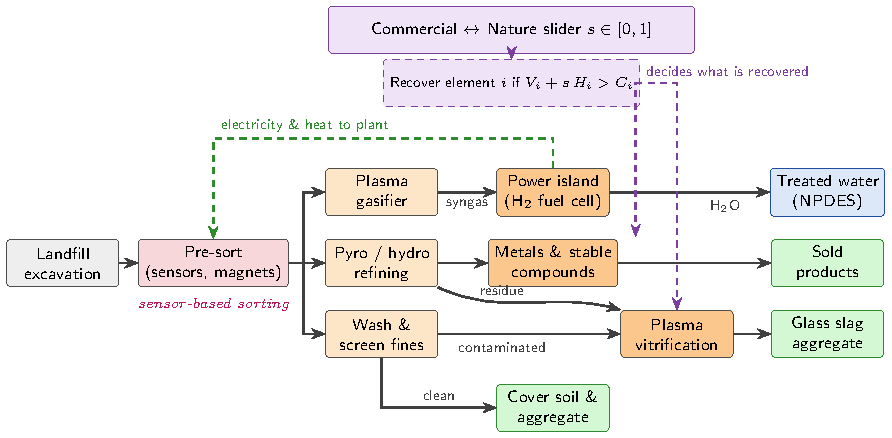
\includegraphics{fig_process.pdf}
\caption{The Sort-First baseline modelled in the spreadsheet.}
\end{figure}
\begin{center}
\small
\begin{tabular}{@{}lrrr@{}}
\toprule
\textbf{Per wet tonne (illustrative inputs)} & \textbf{Commercial $s=0$} & \textbf{Balanced $s=0.5$} & \textbf{Nature $s=1$} \\
\midrule
Elements recovered & 15 & 19 & 20 \\
Recovered products (kg) & 35.9 & 36.0 & 36.3 \\
Vitrified slag (kg) & 88.6 & 219.8 & 350.9 \\
Electricity demand (kWh) & 264.5 & 403.6 & 542.6 \\
Net electricity (kWh) & +208.0 & +68.9 & $-$70.1 \\
Net operating margin (\$) & 51.50 & 42.48 & 29.77 \\
Monetized harm avoided (\$) & 113.01 & 227.76 & 230.91 \\
\bottomrule
\end{tabular}
\end{center}
\begin{center}
\small
\begin{tabular}{@{}>{\raggedright\arraybackslash}p{3.2cm}>{\raggedright\arraybackslash}p{5.5cm}>{\raggedright\arraybackslash}p{5.6cm}@{}}
\toprule
& \textbf{Sort-First (baseline)} & \textbf{Atomize-First (PARAMANU)} \\
\midrule
Input & sorted streams & residue after optional pre-treatment \\
Separates & objects and materials & atoms \\
Separation physics & magnetism, density, optics, chemistry & condensation temperature, mass, chemistry \\
Off-gas & cleaned and released through a stack & none: sealed, closed-mass outlets \\
Toxic elements & captured where chemistry allows & Zn, Cd, Pb condense far from precious metals; Hg to a trap \\
Trace elements & lost when too dilute & concentrated with the band metal (Au 28-fold) \\
Energy (MWh/t) & 0.26--0.54 & 2.9 (all gas) to 10.5 (full atomization), gross \\
Maturity & commercial components & research concept \\
\bottomrule
\end{tabular}
\end{center}

%=====================================================================
\section{Safety and Scope}
%=====================================================================
\textbf{No process stack is not zero impact}: the impact moves to the power plant and to wherever the fuel gas is burned, so every environmental claim needs a life-cycle assessment (ISO 14040/14044 \citep{iso14040,iso14044}). The electricity dominates: at 2.9--6.7\,MWh per tonne, unabated gas combined-cycle power (life-cycle median about 490\,g CO\textsubscript{2}/kWh \citep{schlomer2014}) means about 1.4--3.3\,t CO\textsubscript{2} per tonne of waste, more than landfilling or incineration; nuclear or wind power (about 12\,g/kWh) means about 0.03--0.08\,t. PARAMANU is an environmental gain only on low-carbon power. \textbf{Pressure and containment}: relief only into closed volumes, never to air; torch power interlocked on pressure and wall temperature. \textbf{Excluded from scope, deliberately}: nuclear materials (uranium, thorium, plutonium, neptunium, americium), radium, polonium and radioactive isotopes of sealed sources (tritium, cobalt-60, strontium-90, caesium-137, iridium-192), for security reasons and because they are not expected in meaningful amounts; portal monitors divert discrete items that emit penetrating radiation (not alpha-only sources such as smoke-detector americium). Because the process fractionates every element, natural uranium and thorium are expected to concentrate in Band A and lead-210 and polonium-210 in the cold bands; this is not simulated, so a mass balance and band monitoring are required before operation, and whether any band approaches the U.S. source-material threshold \citep{nrc10cfr40} must be measured. \textbf{Process hazards} include fuel gas and air ingress, nickel and iron carbonyls at the cold end, pyrophoric metal fume, HCl and HF in the condensate, carbon monoxide and torch power; a HAZOP is required. Isotope separation is outside the scope.

%=====================================================================
\section{How the Numbers Were Computed}\label{ch:computing}
%=====================================================================
\paragraph{Software.} Python 3.10 with exactly pinned versions: Cantera 3.2.0, NumPy 2.2.6, SciPy 1.15.3, pandas 2.3.3, matplotlib 3.10.9, pytest 9.1.1. Pinning matters: with newer versions (SciPy 1.17, NumPy 2.4, pandas 3.0) some sweep feeds stalled that finish in about 20\,s with these. A code fingerprint (a hash of every code and data file, printed in \texttt{Results.txt}) identifies exactly which code produced the published results.

\paragraph{Where it ran.} Everything except the two large runs runs on an ordinary computer: the full set of experiments takes about 1.5 hours on the 2-core workstation used to write the paper. The 5,000-feed sweep (570,000 equilibrium states) and the adversarial search (6,656 more ladders) ran on rented cloud servers (RunPod). One script, \texttt{cluster/runpod/run\_on\_runpod.sh} (or \texttt{run\_job\_on\_runpod.sh} for any script), creates a server, uploads the code, runs the tests and the job, downloads the results and shuts the server down, also on error. GPU servers were rented only because they come with many CPU cores; the work itself is CPU work, because each feed is a chain of dependent equilibrium solutions.

\paragraph{Times and costs.} Final sweep: 10 cores, 0.41\,h, about 12,300 feeds per hour, about 3 core-seconds per feed, under one US dollar. Adversarial search: 74 minutes. A 50\,K-step ladder takes about 3 core-seconds on a server core and 10--20\,s on a laptop core.

\paragraph{Lessons from running it.}
\begin{itemize}
\item \textbf{Count the cores you are allowed, not the cores you see.} One server reported 256 host cores but its container was allowed about 31; starting 256 workers made it thrash. The code now reads the container's quota (cgroup) and runs one worker per allowed core, each with one numerical thread.
\item \textbf{Save every result immediately.} Each finished feed is appended to a checkpoint file, so a crashed or interrupted sweep resumes where it stopped, and timestamped STATUS lines show progress and whether a run died.
\item \textbf{Never wait forever.} A feed that takes more than ten minutes is recorded as a failure (none did), so one bad input cannot stall or silently shrink a sweep.
\item \textbf{Every feed is reproducible on its own}: it is defined only by the configuration and its number, through a random stream seeded with both.
\item \textbf{Keep secrets out.} Server and repository keys live only in local files that are never committed; every publication of the code is scanned for them.
\end{itemize}

%=====================================================================
\section{Refining Each Band}\label{ch:refining}
%=====================================================================
Condensation produces concentrates, not pure products. Each band goes to an established route:
\begin{description}
\item[Band A (W, Ti, part of Si and Nd).] Refractory carbides and oxides: tungsten and titanium carbide to hard-metal recyclers or oxide processing.
\item[Band B (Fe with Au, Pd, Pt, Co; Al and Ca oxides).] Smelt, then electrorefine; the precious metals report to the anode residue, from which refiners recover them \citep{cui2008}. The oxides go to slag.
\item[Band C (Mg, Si, Ni, Cu, Cr, Sn, Sb, Ga; the rest of the Au).] Copper and nickel separate by condensation (about 3.5 stages, Result~4) or electrochemically; gold follows copper to copper smelting and precious-metal refining.
\item[Band D1 (S, Mn; tails of Cu, Sn, Sb, Cr, Ga; stray gold in organic-rich feeds).] Route with Band C to copper smelting. Keep separate from D2.
\item[Band D2 (Na, K, Cl salts; Ag, Bi, most of the Pb).] Leach the salts (a product); recover silver and lead from the residue.
\item[Band E (Zn, Cd, In, Li, F, P; the rest of the Pb).] Zinc and cadmium separate by condensation (about 5 stages); cadmium is stored as sulfide, zinc sold as metal (plasma fuming of steel-mill dust recovers about 92\% \citep{cusano2017bref}).
\item[Cold end and trap.] Water; mercury as mercury sulfide from the sulfur-impregnated carbon bed.
\item[Gas.] Methane or H\textsubscript{2} and CO, with N\textsubscript{2}: fuel, after the cold-end gas cleaning of Chapter~\ref{ch:catalysts}; argon recycled.
\item[Everything else.] What the slider does not select is vitrified; toxic products are converted to the stable forms of the storage table.
\end{description}

%=====================================================================
\section{Why Each Prediction and Its Passing Mark}\label{ch:prereg}
%=====================================================================
A passing mark must be tight enough that failing it means something, and loose enough that honest measurement error does not fail a correct model. The reasoning for each:
\begin{description}
\item[P1, element balance.] Result~1 is exact, so the only allowance is measurement uncertainty (3 standard uncertainties). If it fails, the experiment has a leak or an analytical error, and no other prediction can be judged until it is fixed.
\item[P2, energy $\ge$2.90\,MWh/t, fail below 2.6.] 2.90 is a thermodynamic \emph{minimum}; no real device can beat it. The 10\% margin covers errors in measuring the energy delivered. A measurement well below the minimum would mean the thermochemical data are wrong.
\item[P3, iron metallic $\ge$90\%, fail below 50\%.] The model says 100\% with the waste's organics and 43\% without. Below 50\% would mean the internal reductant does not work as equilibrium says, which is the premise of metal bands.
\item[P4, order and $\pm$150\,K.] The order is the core of the ladder; a reversal of zinc, cadmium or mercury above gold or copper would break the separation claim. The 150\,K allowance covers the 50--100\,K shifts that alloying causes for copper and the data differences found with the second database.
\item[P5, no Zn, Hg, Pb in gold bands ($<$1\%).] The central separation claim, never violated in 5,000 random and 6,656 adversarial feeds. The 1\% line is the same threshold the adversary used.
\item[P6, cadmium $<$0.1\%.] The model's maximum is 0.025\%; four times that is still a clear pass, ten times would not be.
\item[P7, gold in B+C $\ge$95\%, fail below 90\%.] The model says 100\%, with a 5th percentile of 99.3\% over the 1\,atm feeds.
\item[P8, gold in B 20--95\%.] Deliberately wide, because this number rests on the weakest datum (gold in liquid iron): the sweep gives 40--83\% at 1\,atm and the coefficient extremes 36--82\%. If it fails, P11 says why.
\item[P9, Pd and Pt with iron $\ge$90\%.] The model says about 100\% (95\% and 94\% of all feeds, the rest in Band A at 5\,atm).
\item[P10, the pressure effect.] Result~3 predicts the sign from $yP$ with no free parameter: raising the pressure must raise gold's condensation temperature and its share in Band B.
\item[P11, gold's activity coefficient in iron 0.5--7.] The model uses 1.4--2.3 near 2,000--2,250\,K, extrapolated; the range allows a factor of about three either way, like the uncertainty assumed for unmeasured pairs. Outside it, the model is rerun with the measured value, as declared in advance.
\item[P12, CF\textsubscript{4} $<$0.01\% leaves the hot zone.] At 2,600\,K the Damk\"ohler number is 53, so equilibrium chemistry predicts destruction far below this. If more leaves, the hot zone is not uniform (cold parcels near the walls) or the rate data are wrong.
\item[P13, the adversary's feed: gold in D1, lead in D2.] The design change the search forced is itself tested: the organic-rich feed on which the first design failed must show the separation the split was made for.
\end{description}

%=====================================================================
\section{What Is Proven, What Is Verified, What Is Open}\label{ch:feasibility}
%=====================================================================
\begin{description}
\item[Tier 1, mathematical proof.] Results 1--4 and 6--8 are established results of thermodynamics and convex optimization, applied here; Result 5 is an order-of-magnitude estimate built on a rigorous geometric bound. A critic can dispute their assumptions (ideal gas, equilibrium, pure phases or ideal solutions) for a real reactor, not their conclusions.
\item[Tier 2, verified computation.] What thermodynamics predicts for this waste, computed correctly: it rests on NASA and NIST-JANAF data \citep{chase1998} (most trusted), measured activity coefficients (weakest; one of them decides gold's split) and the standard CEA method; and it is checked by the certificate, a second solver and database, the adversary, Sobol indices and a second machine.
\item[Tier 3, not yet proven.] That a real reactor behaves like the equilibrium model. Five gaps: \emph{fume and aerosols} (fast-cooled metal vapor nucleates into particles that can be carried past their condenser, probably the largest threat to band purity; not modelled); \emph{kinetics and nucleation} (not modelled); \emph{non-ideal alloys and slag} (bracketed); \emph{a hot zone of 25\,ms at scale} (sized, not demonstrated); \emph{energy efficiency} (2.9\,MWh/t is a minimum; best demonstrated 2.3$\times$).
\end{description}
\textbf{The claim}, therefore, is \emph{thermodynamic feasibility with a verified computation}, not a working plant. \textbf{The experiment that decides}: a sealed arc furnace or plasma torch, a few kilograms of synthetic residue made to \texttt{feed.py}, and condensers at the band temperatures, within reach of a university laboratory, testing P3 (iron as metal), P4 (order of condensation) and P5 (no zinc, mercury or lead with the gold). \emph{The mathematics is proof, the computation is verified evidence, and the working plant awaits experiment.}

%=====================================================================
\section{Research Agenda}
%=====================================================================
\begin{description}
\item[R1] Metals or oxides? Sealed bench arc furnace, synthetic residue, analyse each collector (ICP-MS, X-ray diffraction) at several cooling rates.
\item[R2] How clean is each band? Cross-contamination, co-condensation, salts, aerosols.
\item[R3] Can a plasma mass filter split co-condensing groups?
\item[R4] Can the hot zone be built? Sealed flow reactor with condensers; residence time, wall losses, the three flow conditions.
\item[R5] Energy: transferred-arc or centrifugal furnace against powder injection; heat recovery.
\item[R6] Pre-treatment at 0, 15 and 30\%: output quality unchanged?
\item[R7] Real-time monitoring by optical emission spectroscopy.
\item[R8] Scale-up from 1\,kg to 1\,t batches.
\item[R9] The model: done in this work, full trace chemistry, benchmarks and verification; next, measure gold's activity coefficient in liquid iron (P11), CALPHAD solution models, nucleation, aerosols and reacting-flow simulation.
\end{description}

%=====================================================================
\section{The Pre-Publication Review}\label{ch:review}
%=====================================================================
Before submission the paper was audited three ways, independently: every number against the result files; every claim and proof as a demanding referee would read it; and every reference against Crossref and, where accessible, the source itself. About 100 findings were checked and fixed. The substantive ones:
\begin{description}
\item[Zinc and lead in the gold bands.] The ``none in 5,000 feeds'' result holds for pure condensed metals, the setting of the sweep, in which zinc and lead cannot dissolve in iron or copper. The paper now says so and gives the ideal-alloy values (0.009\% zinc, 0.5\% lead) and notes that non-ideal copper alloys need a CALPHAD check.
\item[Scope of the certificate.] It certifies the major-element equilibrium; the trace metals, gold included, are placed by the separately tested dilute-limit solver. Stated explicitly.
\item[Caveats in the abstract.] Local equilibrium, pure oxide phases, no nucleation or aerosol carry-over, no slag solution, no torch-gas dilution: now in the abstract, with torch-gas dilution quantified (above).
\item[The lead fix has a wide margin.] Recomputed in 12.5\,K steps, the worst adversarial feed has 99.9\% of its gold condensed by 1,575\,K and its first 0.1\% of lead at 1,025\,K: the 1,300\,K split sits in a 550\,K gap.
\item[Hot-zone basis.] The sizing mixed per-kilogram values of the reactor feed (961\,kg) with a throughput of excavated material; now per excavated tonne: 96\,m\textsuperscript{3}/s (was 100), 119/126\,MW (was 124/130).
\item[Radioactive materials.] The paper no longer says they stay dispersed: a fractionating process will redistribute natural uranium and thorium (to Band A) and lead-210 and polonium-210 (to the cold bands); a mass balance and band monitoring are required before operation.
\item[Wording.] ``Nothing escapes'' became ``no process gas is vented; every stream leaves through a labelled outlet''; ``thermodynamic minimum'' became ``gross enthalpy without heat recovery''; ``plasma heap'' is defined as a torch-heated vapor; the subtitle now says ``Sealed Plasma Reactor'' because the design is a flow, not a slowly cooled batch; Result~5 is called an order-of-magnitude estimate; Result~6 bounds unmixing, not reduction; the economics are stated as not assessed and likely unfavourable at demonstrated efficiencies.
\item[Safety.] A process-hazards paragraph was added: fuel gas and air ingress, nickel and iron carbonyls at the cold end, pyrophoric metal fume, HCl and HF in the condensate, carbon monoxide, torch power.
\item[References.] A wrong source for mercury capture was replaced (Korpiel \& Vidic 1997); the steel-dust benchmark now says its main reductant was spent mushroom substrate and the comparison uses the coke runs; the EU mercury law, flash Joule heating, the silica-vaporization efficiencies, the glass-dissolution figure and eight other sentences were corrected to what their sources say; bibliography metadata fixed.
\item[Final consistency audit.] A last independent pass over the finished paper found 20 leftovers from before the revision, all fixed: a stale gas flow in the safety paragraph, lead described as condensing ``at the cold end'', the batch-cycle algorithm still written with the first-guide bands and a ``hold'' step (now one parcel through bands A--E in milliseconds), ``time-domain'' and ``sealed batch'' wording where the design is a flow, rounding in the landfill inventory, the energy ratio to the baseline (5--11 times, 40 only for full atomization), and the pure-phase qualifier in two places. The torch-gas dilution and the 550\,K margin of the Band D split were given their own script (\texttt{22\_dilution\_and\_margin.py}) and a section in \texttt{Results.txt}, so that every number in the paper can be regenerated from the code.
\item[Condensed paper.] The paper was condensed from 57 to 18 pages. It keeps all eight Results with their proofs, the certificate, the verification findings, the pre-registered predictions and the energy and self-sufficiency account. The longer explanations, the implementer's guide, the catalyst tables, the full landfill inventory and the extra figures moved here. The earlier full-length version is kept by the author.
\item[Pre-registration.] The file is to be deposited with a timestamped DOI at submission; the consistency checks (P1, P2) are now distinguished from the risky predictions (P3--P13).
\end{description}

%=====================================================================
\section{How the Work Developed}
%=====================================================================
\begin{description}
\item[28 September 2026.] The paper began as a Sort-First design with a mass-energy spreadsheet, became Atomize-First, gained the open simulation and its evidence, and then the mathematical results. Critics' first objection, ``a vision needs evidence'', shaped the simulation.
\item[29 September 2026.] The 5,000-feed Monte Carlo sweep was moved to rented cloud servers; trace metals got full chemistry with chlorides and measured activity coefficients; benchmarks against published measurements; how complex waste comes apart; the chamber walkthrough; the landfill inventory and long-term storage; the catalyst chapter; then the rechecking of the computation, which found and fixed three solver defects and one design flaw (below); Sobol indices, reproducibility, pre-registration; and the feasibility proof.
\end{description}

\paragraph{Corrections that changed results} (the full, dated log is at the end of \texttt{Results.txt}):
\begin{enumerate}
\item \textbf{Rule-of-three denominator.} The first analysis divided by all 5,000 feeds, but only 971 contained zinc and lead (the soil had none), so the claimed 0.06\% bound was really 0.31\%. Fixed by counting only feeds containing the metal and by giving the soil its measured heavy metals \citep{vollprecht2020}, so every feed contains them. \emph{Lesson: always ask what the denominator is.}
\item \textbf{Two faulty data records} (PtH, SbF) rejected by checking every record against its own heat of formation.
\item \textbf{Unconverged solver steps} (43 of 229): dilute-element split.
\item \textbf{Cantera's false convergence} at 0.1\,atm: the certificate; the affected sweep rerun.
\item \textbf{Missing graphite} in rare states: the CEA phase-set loop.
\item \textbf{Lead in Band D} (the adversary): Band D split at 1,300\,K; sweep and search rerun.
\end{enumerate}

%=====================================================================
\section{Where Everything Is}
%=====================================================================
\begin{center}
\small
\begin{tabular}{@{}>{\raggedright\arraybackslash}p{4.6cm}>{\raggedright\arraybackslash}p{10cm}@{}}
\toprule
\textbf{Path} & \textbf{Contents} \\
\midrule
\texttt{README.md} & overview and start here \\
\texttt{AllExplainedHere.pdf} & this document \\
\texttt{Results.txt} & every result, generated from the code; code fingerprint; corrections log \\
\texttt{HOWTOREPLICATE.txt} & step by step, from a fresh computer to the same numbers \\
\texttt{paper/} & the paper's LaTeX source, figures, bibliography; \texttt{build.sh} builds PDF, HTML, Word \\
\texttt{simulation/paramanu\_sim/} & the model (Chapter~\ref{ch:code}) and its data \\
\texttt{simulation/scripts/} & experiments 01--23 \\
\texttt{simulation/results/} & CSV results, figures, \texttt{key\_numbers.json}, the 5,000-feed table \\
\texttt{simulation/tests/} & 38 automated tests \\
\texttt{simulation/cluster/runpod/} & run the sweep or any script on a rented cloud server \\
\texttt{docs/STUDENT\_GUIDE.md} & redo every proof and check, with exercises \\
\texttt{docs/IMPLEMENTERS\_GUIDE.md} & design procedure, command by command \\
\texttt{docs/PREREGISTRATION.md} & the 13 predictions, fixed in advance \\
\texttt{docs/all\_explained/} & the source of this document \\
\texttt{model/} & the Sort-First baseline spreadsheet and its generator \\
\bottomrule
\end{tabular}
\end{center}

\paragraph{The experiments.} 01 validation; 02 ladder; 03 reductant; 04 energy; 05 chamber; 06 sweep; 07 theory checks; 08 reactor design; 09 convergence; 10 sensitivity; 11 alloying; 12 sweep analysis; 13 breakdown; 14 benchmarks; 15 gold between iron and copper; 16 landfill inventory; 17 catalysts; 18 second solver and database; 19 reproducibility; 20 adversarial search; 21 Sobol indices. \texttt{run\_all.sh} runs them and regenerates \texttt{Results.txt}.

%=====================================================================
\section{Questions Critics Ask}
%=====================================================================
\begin{description}
\item[Is it really a plasma?] No: at 2,890\,K the heap is 0.02\% ionized, a hot vapor heated by plasma torches. The paper says so.
\item[How do you know the solver is right?] Every state passes a certificate derived from Result~2 that does not trust the solver; a second, independent solver and a second database agree; results reproduce on another machine to $10^{-13}$.
\item[Did you only test typical cases?] No: an optimizer searched 56 inputs for failures, found one (lead), and the fixed design survived a full second search.
\item[What if the real reactor is not at equilibrium?] Then the model's numbers are an ideal the plant approaches; the benchmarks show equilibrium is the ceiling that a gas-phase reductant reaches. Kinetics, nucleation and aerosols are named as the main unknowns (Tier 3) and are the first experiments.
\item[Can condensation separate gold from iron?] No, and the paper does not claim it (26 stages, Result~4). Gold follows iron and copper into alloys that existing refineries process.
\item[Isn't the energy too high?] 2.9\,MWh/t minimum, about 2.3$\times$ that in the best device demonstrated: a dedicated power plant is required, and the environmental case depends on its electricity.
\item[Can a catalyst make it cheaper?] Not in the hot zone (Result~8, and none survives); at the cold end, yes, for gas cleaning.
\item[What about dioxins and PFAS?] CF\textsubscript{4}, the hardest PFAS end product, lives 75\,\textmu s at 2,900\,K against a 25\,ms hot zone; dioxin re-formation is avoided by a fast quench through 450--200\,\textdegree C and a catalytic filter.
\item[What about radioactive material?] Excluded from scope; diverted at intake to licensed handlers.
\item[Why should I believe you did not tune the model to the answer?] Everything is public with pinned versions and step-by-step instructions; the corrections are logged with dates; and the predictions for the first experiments are fixed in advance.
\end{description}

\appendix
%=====================================================================
\section{The Implementer's Guide, Step by Step}\label{app:guide}
%=====================================================================
The paper's Appendix~A turns the results into a design procedure; the command-by-command version is \texttt{docs/IMPLEMENTERS\_GUIDE.md}. Each step: what to do, which result or program, and the worked example for 1,000 wet tonnes per day at 1\,atm with the default feed. Replace every default with site data.
\begin{description}
\item[A.1 Characterize the feed.] Composite samples across depth and area; moisture, loss on ignition (organic content), major elements by X-ray fluorescence, traces by ICP-MS. Enter component masses and trace concentrations in \texttt{feed.py}. \emph{Example:} 250\,kg water and 711\,kg dry residue per wet tonne; soil as upper-crust oxides.
\item[A.2 Make hazards safe (mandatory).] Discharge and dismantle batteries; depressurize cylinders and aerosol cans; divert anything flagged by radiation portal monitors to a licensed handler.
\item[A.3 Compute the all-gas state.] Run \texttt{04\_energy.py}: all-gas temperature $T$, specific energy $e$ and gas yield $\nu$ at the chosen pressure. \emph{Example:} 2,890\,K, 9.8\,MJ/kg and 35.1\,mol/kg of excavated material (drying excluded).
\item[A.4 Choose the pressure.] Higher pressure raises the all-gas temperature slightly (3,190\,K at 10\,atm), shrinks the hot volume and helps mercury condense (22\% left in the gas at 2\,atm against 51\% at 1\,atm for the default feed); lower pressure lowers the all-gas temperature (2,630\,K at 0.1\,atm) but moves gold toward colder bands. \emph{Example:} 1\,atm in the hot zone; 2\,atm or more at the mercury trap.
\item[A.5 Size the hot zone.] Choose the allowed radiation loss and solve Result~5 for the residence time $t_r$; torch power $\dot W = \dot m e/(1 - Q/\dot W)$; hot volume $V = \dot m\,\nu RT t_r/P$. \emph{Example:} $\dot m = 11.57$\,kg/s, 96\,m\textsuperscript{3}/s of gas; 5\% loss: 10\,ms, 1.0\,m\textsuperscript{3}, 119\,MW; 10\% loss: 25\,ms, 2.4\,m\textsuperscript{3}, 126\,MW. A batch design must instead heat and quench each batch in a small fraction of its time constant.
\item[A.6 Design the condenser train.] Run \texttt{02\_ladder.py} with site data; one collector per band, placed along the gas path at the band temperatures; size each exchanger from its duty $\dot Q$ with $A = \dot Q/(U\,\Delta T_{\mathrm{lm}})$. Where a band must be split further, Result~4 gives the minimum stages. \emph{Example:} 13.6, 28.3, 21.9, 3.3, 11.5, 15.7 and 5.4\,MW for A, B, C, D1, D2, E and the cold trap; 42\% of the heat above 2,000\,K, worth recovering.
\item[A.7 Capture mercury.] A sulfur-impregnated carbon bed after the coldest collector, sized for the full mercury input, since up to all of it may arrive; check the mercury balance on every campaign.
\item[A.8 Route each band to refining.] Chapter~\ref{ch:refining}. Keep D1 and D2 in separate collectors.
\item[A.9 Acceptance tests.] (1) Every element balance closes within measurement error; (2) the onset of each metal collected as a pure phase lies within the bounds of Result~3; (3) band compositions agree with the model for the measured feed, any disagreement explained by alloying or kinetics; (4) mercury at the outlet below the permit limit; (5) energy per tonne and radiation loss agree with Results~5 and~6. The pre-registered predictions (Chapter~\ref{ch:prereg}) are the research version of these tests.
\item[A.10 Safety.] Relieve pressure only into closed volumes, never to air; interlock torch power on vessel pressure and wall temperature; radiation portal monitors at intake; the relevant permits (water discharge, hazardous-waste rules).
\end{description}

%=====================================================================
\section{Catalogue of Experiments}\label{app:scripts}
%=====================================================================
Every number and figure comes from one of these scripts in \texttt{simulation/scripts/}. The first line of each script's own description:
\input{tables/scripts}
\noindent What each produces, in brief:
\begin{description}
\item[01 validate] boiling points of 15 elements and gas mixtures against Cantera (Chapter~\ref{ch:results}).
\item[02 ladder] the default ladder: band shares, $T_{10/50/90}$, band masses, species, figures.
\item[03 reductant] the ladder with organics $\times$0, 0.5, 1, 2.
\item[04 energy] the energy curve and envelope by pressure and pre-treatment.
\item[05 chamber] batch volume, radiation, Saha ionization (GPU-capable).
\item[06 sweep] the Monte Carlo sweep (resumable; cloud-ready).
\item[07 theory checks] Results 3, 4, 6 against the simulation.
\item[08 reactor design] Result 5: batch time constant, flow loss, condenser duties.
\item[09 convergence] the ladder at 100, 50, 25, 12.5\,K steps.
\item[10 sensitivity] one-at-a-time changes.
\item[11 alloy model] the ideal liquid-metal alloy.
\item[12 sweep analysis] each claim over the sweep, rule-of-three bounds, by pressure.
\item[13 breakdown] Result 7 and how complex waste comes apart.
\item[14 benchmarks] vapor pressures; steel-mill dust.
\item[15 gold copper] gold between iron and copper: benchmark and ladder scenarios.
\item[16 landfill inventory] pounds per element in the median US landfill.
\item[17 catalysts] catalyst survival, Damk\"ohler numbers, carbon as reagent.
\item[18 independent verification] second solver and second database.
\item[19 reproducibility] sweep feeds recomputed on another machine.
\item[20 falsification] the adversarial search.
\item[21 global sensitivity] Sobol indices from the sweep.
\item[22 dilution and margin] torch-gas dilution; margin of the Band D split.
\end{description}
\texttt{simulation/run\_all.sh} runs them in order and regenerates \texttt{Results.txt} with \texttt{tools/write\_results.py}.

%=====================================================================
\section{Catalogue of Automated Tests}\label{app:tests}
%=====================================================================
\texttt{pytest} in \texttt{simulation/} runs these 24 test functions, 38 cases in all (some run for several elements or conditions). They check the physics (element conservation, uniqueness, boiling points, the closed-form results), the data (every thermochemical record against its own stated heat of formation), the method (the dilute limit against the full solver, every ladder state certified) and the machinery (checkpoint and resume, CPU detection). They run on every change, and on the cloud server before every sweep.
\input{tables/tests}

%=====================================================================
\section{Replicating Everything: The Short Version}
%=====================================================================
\begin{enumerate}
\item \texttt{git clone https://github.com/syncaissa/paramanu-reclaimer.git}; Python 3.10; \texttt{pip install -r simulation/requirements.txt} (exact versions).
\item \texttt{cd simulation \&\& pytest}: expect 38 passed.
\item \texttt{python tools/write\_results.py --fingerprint}: compare with \texttt{Results.txt}.
\item \texttt{cd scripts \&\& python 01\_validate.py \&\& python 02\_ladder.py}: 10 minutes; compare with \texttt{Results.txt} sections 1--2 (gold 58.1\% B / 41.9\% C; T50 Fe 2,225\,K).
\item \texttt{./run\_all.sh}: every experiment, about 1.5 hours.
\item The 5,000-feed sweep on a many-core machine or a rented server (\texttt{SAMPLES=5000}); then scripts 12, 21 and 19.
\item Regenerate \texttt{Results.txt} and compare with the published one; any difference other than dates is worth reporting.
\end{enumerate}
The full instructions, with expected outputs and troubleshooting, are in \texttt{HOWTOREPLICATE.txt}.

\bibliographystyle{apalike}
\bibliography{../../paper/references}

\begin{pclosing}
Syncaissa Systems Inc. \quad $\bullet$ \quad \texttt{syncaissa@outlook.com}\\[2pt]
\url{https://github.com/syncaissa/paramanu-reclaimer}
\end{pclosing}

\end{document}
